% ------------------------------------------------------------------------
%  My Format for a Article
% ------------------------------------------------------------------------
\documentclass[12pt]{article}
\oddsidemargin 0.0in
\textwidth 6.5in
\textheight 9in
\topmargin -0.35in
\headheight 0.0in
\hfuzz 10pt

\renewcommand{\thefootnote}{\fnsymbol{footnote}}
\newcommand{\be}{\begin{equation}}
\newcommand{\ee}{\end{equation}}
\newcommand{\Curl}{\nabla \times}
\newcommand{\Div}{\nabla \cdot}

% ------------------------------------------------------------------------
% Definitions so that LaTeX won't throw a
% "Too many unprocessed floats" tantrum
% ------------------------------------------------------------------------
\renewcommand{\topfraction}{.85}
\renewcommand{\bottomfraction}{.7}
\renewcommand{\textfraction}{.15}
\renewcommand{\floatpagefraction}{.66}
\renewcommand{\dbltopfraction}{.66}
\renewcommand{\dblfloatpagefraction}{.66}
\setcounter{topnumber}{9}
\setcounter{bottomnumber}{9}
\setcounter{totalnumber}{20}
\setcounter{dbltopnumber}{9}

% ------------------------------------------------------------------------
% Packages to use for a dvips document:
% ------------------------------------------------------------------------
\usepackage{pslatex}
\usepackage[dvips]{graphicx}
\usepackage[dvips]{hyperref}
\begin{document}

% ------------------------------------------------------------------------
% Title Page:
% ------------------------------------------------------------------------
\thispagestyle{empty}

\vspace*{2.5in}

\vspace*{0.5in}
\begin{center}
{\LARGE Finite Element Method Magnetics: OctaveFEMM}

\vspace*{16pt} {\Large Version 1.2}

\vspace*{16pt} {\Large User's Manual}

\vspace*{16pt} \today

\vspace*{48pt} David Meeker \\
\href{mailto:dmeeker@ieee.org}{\tt dmeeker@ieee.org} \\
\href{http://femm.foster-miller.com}{\tt http://femm.foster-miller.com} \\
\copyright 2006
\end{center}

\newpage


% ------------------------------------------------------------------------
% Main Text:
% ------------------------------------------------------------------------
\section{Introduction}

OctaveFEMM is a Matlab toolbox that allows for the operation of Finite
Element Method Magnetics (FEMM) via a set of Matlab functions.  The toolbox
works with Octave, a Matlab clone.

When OctaveFEMM starts up a FEMM process, the usual FEMM user interface
is displayed and is fully functional.  The user then has the choice of
accomplishing modeling and analysis tasks either exclusively through
functions implemented by the toolbox, or by a combination of manual and
programmatic operations -- whichever is easiest for the task at hand.

The syntax of the OctaveFEMM toolbox closely mirrors that of FEMM's existing
Lua scripting language interface associated with FEMM v4.2.  However, there
are some differences between the Lua functions and the analogous Octave/Matlab
implementations:
\begin{itemize}
\item All strings are enclosed in single quotes, rather than
double quotes as in Lua.
\item Functions in Lua that have no arguments require a set of
empty parentheses after the function name ({\em e.g.} {\tt
mi\_analyze()}).  In Octave or Matlab, no parentheses should be used needed ({\em e.g.} {\tt
mi\_analyze} with the OctaveFEMM toolbox).
\item Several commands have also been added to OctaveFEMM that have no
analog in Lua.  These commands streamline the drawing of new
geometries with the OctaveFEMM toolbox, as well is the collection
of data from solutions.
\end{itemize}

Perhaps the most remarkable difference between Lua and OctaveFEMM,
however, is due to the matrix-oriented nature of Octave/Matlab.  In just about any
OctaveFEMM function in which it would be desiable to enter an array
of points such that multiple copies of an operation are performed, OctaveFEMM
will correctly interpret the input perform the requested operation
on every element in the array.  In addition, for any function in which
the coordinates of a point are required, that point can be
specified as an array with two elements instead of specifying each
element separately.  In functions that require the specification
of multiple points, those points can be entered as an array of
two-element arrays.

\section{Installation and Startup}

\subsection{Installation for Matlab and Octave 3}
The OctaveFEMM distribution is automatically installed with FEMM 4.2 in the
\verb+mfiles+ subdirectory.  The absolute directory is typically
\verb+c:\Program Files\femm42\mfiles+.  To use OctaveFEMM with Octave or
Matlab, this path needs to be added to the program's search path. To add
this path to the search path, type the following lines at the Matlab or
Octave 3.X.X command prompt:

\begin{verbatim}
	addpath('c:\\progra~1\\femm42\\mfiles');
	savepath;
\end{verbatim}

Alternatively, in Matlab, the interactive {\tt pathtool} command can be used
to add the {\tt mfiles} directory to the search path.

\subsection{Installation for Octave 2.1.50 and Octave 2.1.73}

It is recommended that you use a newer version of Octave that has support
for the {\tt actxserver} function.  If this function exists, Octave will use
ActiveX automation to communication with FEMM.  However, OctaveFEMM can
still be used with versions of Octave ({\em e.g.} Octave 2.1.50 and 2.1.73)
that do not support ActiveX. If {\tt actxserver} is not available, a much
slower interprocess communication mechanism based on temporary files will be
used.

Again, to use OctaveFEMM, the directory where the OctaveFEMM mfiles are located
must be permanently added to the search path.  This directory can be added to
the search path by an appropriate modification of the \verb+.octaverc+ initialization
file. For example, in the
Octave 2.1.50 release, Octave looks for \verb+.octaverc+ in the directory:

\verb+C:\Program Files\GNU Octave 2.1.50\octave_files+

To insert OctaveFEMM into the search path, one can create the {\tt .octaverc file} and
add the line:

\verb+LOADPATH = [ '/cygdrive/c/progra~1/femm42/mfiles//', LOADPATH ];+

to add the directory containing the OctaveFEMM commands to the Octave search path.

\subsection{Startup}
To start an OctaveFEMM session, use the {\tt openfemm} function.
This function starts up a FEMM process to which OctaveFEMM calls
are sent. When done with OctaveFEMM, the FEMM process can be shut
down via the {\tt closefemm} function.

A number of examples that use OctaveFEMM to analyze various problems
are included in the directory \verb+cd c:\Program Files\femm42\examples+

%-----------------------------------------------------------------------------------
%
%  OctaveFEMM Documentation
%
%-----------------------------------------------------------------------------------

% Magnetics-specific functions
% ------------------------------------------------------------------------
%  My Format for a Article

\section{Common Command Set}

There are a number of FEMM-specific Octave that are not associated with any particular problem type.
These functions manipulate the appearance of the main window and
other top-level components like the Lua console and Point
Properties output window.

\begin{itemize}

\item {\tt clearconsole} Clears the output window of the Lua console.

\item {\tt newdocument(doctype)} Creates a new preprocessor document
and opens up a new preprocessor window.  Specify {\tt doctype} to
be {\tt 0} for a magnetics problem, {\tt 1} for an electrostatics
problem, {\tt 2} for a heat flow problem, or {\tt 3} for a current
flow problem. Alternative syntax for this function is {\tt create(doctype)}

\item{\tt hideconsole} Hides the floating Lua console window.

\item{\tt hidepointprops} Hides the floating FEMM Properties display window.

\item \texttt{messagebox('message')} displays the \texttt{'message' }string to the
screen in a pop-up message box.

\item {\tt opendocument('filename')} Opens a document specified by {\tt filename}.

\item \texttt{print(item1,item2,...)} This is standard Lua ``print'' command directed to the
output of the Lua console window. Any number of comma-separated items can be
printed at once via the print command.

\item \texttt{prompt('message')} This function allows a FEMM script to prompt a
user for input. When this command is used, a dialog box pops up with the
\texttt{'message'} string on the title bar of the dialog box. The user can
enter in a single line of input via the dialog box.  Prompt returns the
user's input to Octave and parses it using Octave's {\tt eval}
command.

\item{\tt showconsole} Displays the floating Lua console window.

\item{\tt showpointprops} Displays the floating FEMM Properties
display window.

\item{\tt main\_minimize} minimizes the main FEMM window.

\item{\tt main\_maximize} maximizes the main FEMM window.

\item{\tt main\_restore} restores the main FEMM window from a
 minimized or maximized state.

\item{\tt main\_resize(width,height)} resizes the main FEMM
 window client area to width $\times$ height.

\end{itemize}


\section{Magnetics Preprocessor Command Set}

A number of different commands are available in the preprocessor.

\subsection{Object Add/Remove Commands}

\begin{itemize}

\item{\tt mi\_addnode(x,y)} Add a new node at x,y

\item{\tt mi\_addsegment(x1,y1,x2,y2)} Add a new line segment from node
closest to (x1,y1) to node closest to (x2,y2)

\item{\tt mi\_addblocklabel(x,y)} Add a new block label at (x,y)

\item{\tt mi\_addarc(x1,y1,x2,y2,angle,maxseg)} Add a new arc segment
from the nearest node to (x1,y1) to the nearest node to (x2,y2)
with angle `angle' divided into `maxseg' segments.

\item{\tt mi\_drawline(x1,y1,x2,y2)} Adds nodes at (x1,y1) and
(x2,y2) and adds a line between the nodes.

\item{\tt mi\_drawpolyline([x1,y1;x2,y2'...])} Adds nodes at each
of the specified points and connects them with segments.

\item{\tt mi\_drawpolygon([x1,y1;x2,y2'...])} Adds nodes at each
of the specified points and connects them with segments to form a
closed contour.

\item{\tt mi\_drawarc(x1,y1,x2,y2,angle,maxseg)} Adds nodes at
(x1,y1) and (x2,y2) and adds an arc of the specified angle and
discretization connecting the nodes.

\item{\tt mi\_drawrectangle(x1,y1,x2,y2)} Adds nodes at the
corners of a rectangle defined by the points (x1,y1) and (x2,y2),
then adds segments connecting the corners of the rectangle.

\item{\tt mi\_deleteselected} Delete all selected objects.

\item{\tt mi\_deleteselectednodes} Delete selected nodes.

\item{\tt mi\_deleteselectedlabels} Delete selected block labels.

\item{\tt mi\_deleteselectedsegments} Delete selected segments.

\item{\tt mi\_deleteselectedarcsegments} Delete selects arcs.
\end{itemize}

\subsection{Geometry Selection Commands}

\begin{itemize}
\item{\tt mi\_clearselected} Clear all selected nodes, blocks, segments
and arc segments.

\item{\tt mi\_selectsegment(x,y)} Select the line segment closest to
(x,y)

\item{\tt mi\_selectnode(x,y)} Select the node closest to (x,y).
Returns the coordinates of the selected node.

\item{\tt mi\_selectlabel(x,y)} Select the label closet to (x,y).
Returns the coordinates of the selected label.

\item{\tt mi\_selectarcsegment(x,y)} Select the arc segment closest to
(x,y)

\item{\tt mi\_selectgroup(n)} Select the $n^{th}$ group of nodes, segments, arc
segments and blocklabels. This function will clear all previously selected
elements and leave the editmode in 4 (group)
\end{itemize}

\subsection{Object Labeling Commands}

\begin{itemize}
\item{\tt mi\_setnodeprop('propname',groupno)} Set the selected nodes to
have the nodal property {\tt 'propname'} and group number {\tt groupno}.

\item{\tt mi\_setblockprop('blockname', automesh, meshsize, 'incircuit',
magdir, group, turns)} Set the selected block labels to have the
properties:
\begin{itemize}
\item Block property {\tt 'blockname'}.
\item {\tt automesh}: 0 = mesher defers to mesh size constraint defined in {\tt meshsize},
         1 = mesher automatically chooses the mesh density.
\item {\tt meshsize}: size constraint on the mesh in the block marked by this label.
\item Block is a member of the circuit named {\tt 'incircuit'}
\item The magnetization is directed along an angle in measured in degrees denoted by the parameter
        {\tt magdir}
\item A member of group number {\tt group}
\item The number of turns associated with this label is denoted by {\tt turns}.
\end{itemize}

\item{\tt mi\_setsegmentprop('propname', elementsize, automesh, hide,
group)} Set the selected segments to have:
\begin{itemize}
\item Boundary property {\tt 'propname'}
\item Local element size along segment no greater than {\tt
elementsize}
\item {\tt automesh}:  0 = mesher defers to the element constraint defined by {\tt elementsize},
        1 = mesher automatically chooses mesh size along the selected segments
\item {\tt hide}: 0 =  not hidden in post-processor, 1 == hidden in post processor
\item A member of group number {\tt group}
\end{itemize}

\item{\tt mi\_setarcsegmentprop(maxsegdeg, 'propname', hide, group)} Set the
selected arc segments to:
\begin{itemize}
\item Meshed with elements that span at most {\tt maxsegdeg} degrees per
element
\item Boundary property {\tt 'propname'}
\item {\tt hide}: 0 =  not hidden in post-processor, 1 == hidden in post processor
\item A member of group number {\tt group}
\end{itemize}

\end{itemize}

\subsection{Problem Commands}

\begin{itemize}
\item{\tt mi\_probdef(freq,units,type,precision,depth,minangle,(acsolver))} changes the
problem definition. Set {\tt freq} to the desired frequency in
Hertz.  The {\tt units} parameter specifies the units used for
measuring length in the problem domain.  Valid {\tt 'units'}
entries are {\tt 'inches'}, {\tt 'millimeters'}, {\tt
'centimeters'}, {\tt 'mils'}, {\tt 'meters'}, and {\tt
'micrometers'}. Set the parameter {\tt problemtype} to {\tt 'planar'} for a 2-D
planar problem, or to {\tt 'axi'} for an axisymmetric problem. The
{\tt precision} parameter dictates the precision required by the
solver.  For example, entering {\tt 1E-8} requires the RMS of the
residual to be less than $10^{-8}$.  A fifth parameter, representing the depth of
the problem in the into-the-page direction for 2-D planar problems.  Specify the depth
to be zero for axisymmetric problems. The sixth parameter represents the minimum angle
constraint sent to the mesh generator -- 30 degrees is the usual
choice for this parameter.  The acsolver parameter specifies which solver is to be
used for AC problems: 0 for successive approximation, 1 for Newton.

\item{\tt mi\_analyze(flag)}
runs the magnetics solver.  The {\tt flag} parameter
controls whether the solver window is visible or minimized.  For a
visible window, either specify no value for {\tt flag} or specify
{\tt 0}. For a minimized window, {\tt flag} should be set to {\tt
1}.

\item{\tt mi\_loadsolution} loads and displays the solution corresponding to the
current geometry.

\item {\tt mi\_setfocus('documentname')} Switches the
magnetics input file upon which commands are to act. If
more than one magnetics input file is being edited at a time,
this command can be used to switch between files so that the
mutiple files can be operated upon programmatically. {\tt
'documentname'} should contain the name of the desired document as
it appears on the window's title bar.

\item{\tt mi\_saveas('filename')} saves the file with name {\tt 'filename'}.

\end{itemize}

\subsection{Mesh Commands}

\begin{itemize}
\item{\tt mi\_createmesh} runs triangle to create a mesh. Note that this is not a
necessary precursor of performing an analysis, as {\tt
mi\_analyze} will make sure the mesh is up to date before running
an analysis. The number of elements in the mesh is pushed back onto
the lua stack.

\item{\tt mi\_showmesh} shows the mesh.

\item{\tt mi\_purgemesh} clears the mesh out of both the screen and
memory.
\end{itemize}

\subsection{Editing Commands}

\begin{itemize}
\item{\tt mi\_copyrotate(bx, by, angle, copies )}
        \begin{itemize}
        \item{\tt bx, by} -- base point for rotation
        \item{\tt angle} -- angle by which the selected objects are incrementally
        shifted to make each copy.  {\tt angle} is measured in degrees.
        \item{\tt copies} -- number of copies to be produced from
        the selected objects.
        \end{itemize}

\item{\tt mi\_copyrotate2(bx, by, angle, copies, editaction )}
        \begin{itemize}
        \item{\tt bx, by} -- base point for rotation
        \item{\tt angle} -- angle by which the selected objects are incrementally
        shifted to make each copy.  {\tt angle} is measured in degrees.
        \item{\tt copies} -- number of copies to be produced from
        the selected objects.
        \item{\tt editaction}  0 --nodes, 1 -- lines (segments), 2 --block labels, 3 -- arc
                segments, 4- group
        \end{itemize}

\item{\tt mi\_copytranslate(dx, dy, copies)}
        \begin{itemize}
        \item{\tt dx,dy} -- distance by which the selected objects are incrementally shifted.
        \item{\tt copies} -- number of copies to be produced from the selected objects.
        \end{itemize}

\item{\tt mi\_copytranslate2(dx, dy, copies, editaction)}
        \begin{itemize}
        \item{\tt dx,dy} -- distance by which the selected objects are incrementally shifted.
        \item{\tt copies} -- number of copies to be produced from the selected objects.
        \item{\tt editaction}  0 --nodes, 1 -- lines (segments), 2 --block labels, 3 -- arc
                segments, 4- group
        \end{itemize}

\item{\tt�mi\_createradius(x,�y,�r)}�turns�a�corner�located�at�{\tt�(x,y)}�into�a�curve�of�radius�{\tt�r}.

\item{\tt mi\_moverotate(bx,by,shiftangle)}
        \begin{itemize}
        \item{\tt bx, by} -- base point for rotation
        \item{\tt shiftangle} -- angle in degrees by which the selected objects are rotated.
        \end{itemize}

\item{\tt mi\_moverotate2(bx,by,shiftangle, editaction)}
        \begin{itemize}
        \item{\tt bx, by} -- base point for rotation
        \item{\tt shiftangle} -- angle in degrees by which the selected objects are rotated.
        \item{\tt editaction}  0 --nodes, 1 -- lines (segments), 2 --block labels, 3 -- arc
                segments, 4- group
        \end{itemize}

\item{\tt mi\_movetranslate(dx,dy)}
        \begin{itemize}
        \item{\tt dx,dy} -- distance by which the selected objects are shifted.
        \end{itemize}

\item{\tt mi\_movetranslate2(dx,dy,editaction)}
        \begin{itemize}
        \item{\tt dx,dy} -- distance by which the selected objects are shifted.
        \item{\tt editaction}  0 --nodes, 1 -- lines (segments), 2 --block labels, 3 -- arc
                segments, 4- group
        \end{itemize}

\item{\tt mi\_scale(bx,by,scalefactor)}
        \begin{itemize}
        \item{\tt bx, by} -- base point for scaling
        \item{\tt scalefactor} -- a multiplier that determines how
        much the selected objects are scaled
        \end{itemize}

\item{\tt mi\_scale2(bx,by,scalefactor,editaction)}
        \begin{itemize}
        \item{\tt bx, by} -- base point for scaling
        \item{\tt scalefactor} -- a multiplier that determines how
        much the selected objects are scaled
        \item{\tt editaction}  0 --nodes, 1 -- lines (segments), 2 --block labels, 3 -- arc
                segments, 4- group
        \end{itemize}

\item{\tt mi\_mirror(x1,y1,x2,y2)}
mirror the selected objects about a line passing through the points
{\tt (x1,y1)} and {\tt (x2,y2)}.

\item{\tt mi\_mirror2(x1,y1,x2,y2,editaction)}
mirror the selected objects about a line passing through the points
{\tt (x1,y1)} and {\tt (x2,y2)}. Valid {\tt editaction} entries are
0 for nodes, 1 for lines (segments), 2 for block labels, 3 for arc
segments, and 4 for groups.


\item{\tt mi\_seteditmode(editmode)}
Sets the current editmode to:
        \begin{itemize}
        \item{\tt 'nodes'} - nodes
        \item{\tt 'segments'} - line segments
        \item{\tt 'arcsegments'} - arc segments
        \item{\tt 'blocks'} - block labels
        \item{\tt 'group'} - selected group
        \end{itemize}
This command will affect all subsequent uses of the other editing
commands, if they are used WITHOUT the {\tt editaction} parameter.
\end{itemize}

\subsection{Zoom Commands}

\begin{itemize}
\item{\tt mi\_zoomnatural} zooms to a ``natural'' view with sensible extents.
\item{\tt mi\_zoomout} zooms out by a factor of 50\%.
\item{\tt mi\_zoomin} zoom in by a factor of 200\%.
\item{\tt mi\_zoom(x1,y1,x2,y2)}
Set the display area to be from the bottom left corner specified by
{\tt (x1,y1}) to the top right corner specified by {\tt (x2,y2)}.
\end{itemize}

\subsection{View Commands}

\begin{itemize}
\item{\verb+mi_showgrid+} Show the grid points.
\item{\verb+mi_hidegrid+} Hide the grid points points.
\item{\verb+mi_grid_snap('flag')+}
Setting {\tt flag} to 'on' turns on snap to grid, setting {\tt
flag} to {\tt 'off'} turns off snap to grid.
\item{\verb+mi_setgrid(density,'type')+} Change the grid spacing.  The {\tt density}
parameter specifies the space between grid points, and the {\tt
type} parameter is set to {\tt 'cart'} for cartesian coordinates or
{\tt 'polar'} for polar coordinates.
\item{\tt mi\_refreshview} Redraws the current view.
\item{\tt mi\_minimize} minimizes the active magnetics input view.
\item{\tt mi\_maximize} maximizes the active magnetics input view.
\item{\tt mi\_restore} restores the active magnetics input view from a
 minimized or maximized state.
\item{\tt mi\_resize(width,height)} resizes the active magnetics input
 window client area to width $\times$ height.
%\item{\tt mi\_getview} grabs the currently displayed magnetics input view and imports it into Octave.
\end{itemize}

\subsection{Object Properties}

\begin{itemize}
\item{\tt mi\_addmaterial('matname', mu{\_}x, mu{\_}y, H{\_}c,
J, Cduct, Lam{\_}d, Phi{\_}hmax, lam{\_}fill, LamType, Phi{\_}hx, Phi{\_}hy, nstr, dwire)} adds a
new material with called {\tt 'matname'} with the material
properties:
        \begin{itemize}
        \item{\tt mu{\_}x} Relative permeability in the x- or r-direction.
        \item{\tt mu{\_}y} Relative permeability in the y- or z-direction.
        \item{\tt H{\_}c} Permanent magnet coercivity in
        Amps/Meter.
        \item{\tt J} Applied source current
        density in Amps/mm$^2$.
        \item{\tt Cduct} Electrical conductivity of the material
        in~MS/m.
        \item{\tt Lam{\_}d} Lamination thickness in millimeters.
        \item{\tt Phi\_hmax} Hysteresis lag angle in degrees, used for nonlinear BH curves.
        \item{\tt Lam{\_}fill} Fraction of the volume occupied per lamination that
        is actually filled with iron (Note that this parameter defaults to 1 in the
        {\tt femm} preprocessor dialog box because, by default, iron completely
        fills the volume)
        \item{\tt Lamtype} Set to
                \begin{itemize}
                \item 0 -- Not laminated or laminated in plane
                \item 1 -- laminated x or r
                \item 2 -- laminated y or z
                \item 3 -- magnet wire
                \item 4 -- plain stranded wire
                \item 5 -- Litz wire
                \item 6 -- square wire
                \end{itemize}
        \item{\tt Phi\_hx} Hysteresis lag in degrees in the x-direction for linear problems.
        \item{\tt Phi\_hy} Hysteresis lag in degrees in the y-direction for linear problems.
		\item{\tt nstr} Number of strands in the wire build. Should be 1 for Magnet or Square wire.
		\item{\tt dwire} Diameter of each of the wire's constituent strand in millimeters.
        \end{itemize}
Note that not all properties need be defined -- properties that aren't defined are assigned default
values.


\item{\tt mi\_addbhpoint('blockname',b,h)} Adds a B-H data point the
the material specified by the string {\tt 'blockname'}.  The point to be added
has a flux density of {\tt b} in units of Teslas and a field
intensity of {\tt h} in units of Amps/Meter.

\item{\tt mi\_clearbhpoints('blockname')} Clears all B-H data points
associatied with the material specified by {\tt 'blockname'}.

\item{\tt mi\_addpointprop('pointpropname',a,j)}
adds a new point property of name {\tt 'pointpropname'} with either
a specified potential {\tt a} in units Webers/Meter
or a point current {\tt j} in units of Amps. Set the
unused parameter pairs to 0.

\item{\tt mi\_addboundprop('propname', A0, A1, A2, Phi, Mu, Sig, c0, c1,
BdryFormat)} \\ adds a new boundary property with name {\tt
'propname'}
        \begin{itemize}
        \item For a ``Prescribed A'' type boundary condition, set the {\tt A0,
        A1, A2} and {\tt Phi} parameters as required. Set all other
        parameters to zero.

        \item For a ``Small Skin Depth'' type boundary condtion, set the {\tt Mu}
        to the desired relative permeability and {\tt Sig} to the desired
        conductivity in MS/m.  Set {\tt BdryFormat} to 1 and all other
        parameters to zero.

        \item To obtain a ``Mixed'' type boundary condition, set {\tt C1} and
        {\tt C0} as required and {\tt BdryFormat} to 2.  Set all other
        parameters to zero.

        \item For a ``Strategic dual image'' boundary, set {\tt BdryFormat} to 3
        and set all other parameters to zero.

        \item For a ``Periodic'' boundary condition, set {\tt BdryFormat} to 4 and
        set all other parameters to zero.

        \item For an ``Anti-Perodic'' boundary condition, set {\tt BdryFormat} to
        5 set all other parameters to zero.
        \end{itemize}

\item{\tt mi\_addcircprop('circuitname', i, circuittype)} \\
adds a new circuit property with name {\tt 'circuitname'} with a prescribed current.
The {\tt circuittype} parameter is 0 for a parallel-connected circuit and 1 for a
series-connected circuit.
\item{\tt mi\_deletematerial('materialname')} deletes the material named {\tt
'materialname'}.
\item{\tt mi\_deleteboundprop('propname')} deletes the boundary property named
{\tt 'propname'}.
\item{\tt mi\_deletecircuit('circuitname')} deletes the circuit named {\tt
circuitname}.
\item{\tt mi\_deletepointprop('pointpropname')} deletes the point property named
{\tt 'pointpropname'}
\item{\verb+mi_modifymaterial('BlockName',propnum,value)+} This
function allows for modification of a material's properties without
redefining the entire material ({\em e.g.} so that current can be
modified from run to run).  The material to be modified is
specified by {\tt 'BlockName'}.  The next parameter is the number
of the property to be set. The last number is the value to be
applied to the specified property.  The various properties that can
be modified are listed below:
\begin{center}
\begin{tabular}{lll} \hline
{\tt propnum}& Symbol & Description \\ \hline
 0 & {\tt BlockName} & Name of the material \\
 1 & $\mu_x$ & x (or r) direction relative permeability \\
 2 & $\mu_y$ & y (or z) direction relative permeability \\
 3 & $H_c$   & Coercivity, Amps/Meter \\
 4 & $J$   & Source current density, MA/m$^2$ \\
 5 & $\sigma$ & Electrical conductivity, MS/m \\
 6 & $d_{lam}$  & Lamination thickness, mm \\
 7 & $\phi_{hmax}$ & Hysteresis lag angle for nonlinear problems, degrees \\
 8 & LamFill & Iron fill fraction \\
 9 & LamType & 0 = None/In plane, 1 = parallel to x, 2=parallel to y \\
 10 & $\phi_{hx}$ & Hysteresis lag in x-direction for linear problems, degrees \\
 11 & $\phi_{hy}$ & Hysteresis lag in y-direction for linear problems, degrees \\
 \hline
 \end{tabular}
 \end{center}
\item{\verb+mi_modifyboundprop('BdryName',propnum,value)+}
This function allows for modification of a boundary property. The
BC to be modified is specified by {\tt 'BdryName'}.  The next
parameter is the number of the property to be set. The last number
is the value to be applied to the specified property.  The various
properties that can be modified are listed below:
\begin{center}
\begin{tabular}{lll} \hline
{\tt propnum}& Symbol & Description \\ \hline
 0 & {\tt BdryName} & Name of boundary property \\
 1 & $A_0$ & Prescribed A parameter \\
 2 & $A_1$ & Prescribed A parameter \\
 3 & $A_2$ & Prescribed A parameter \\
 4 & $\phi$ & Prescribed A phase \\
 5 & $\mu$ & Small skin depth relative permeability \\
 6 & $\sigma$ & Small skin depth conductivity, MS/m \\
 7 & $c_0$ & Mixed BC parameter \\
 8 & $c_1$ & Mixed BC parameter \\
 9 & {\tt BdryFormat} & Type of boundary condition: \\
   &                 & 0 = Prescribed A \\
   &                 & 1 = Small skin depth \\
   &                 & 2 = Mixed \\
   &                 & 3 = Strategic Dual Image \\
   &                 & 4 = Periodic \\
   &                 & 5 = Antiperiodic \\ \hline
\end{tabular}
\end{center}
\item{\verb+mi_modifypointprop('PointName',propnum,value)+}
This function allows for modification of a point property. The
point property to be modified is specified by {\tt 'PointName'}.
The next parameter is the number of the property to be set. The
last number is the value to be applied to the specified property.
The various properties that can be modified are listed below:
\begin{center}
\begin{tabular}{lll} \hline
{\tt propnum}& Symbol & Description \\ \hline
 0 & {\tt PointName} & Name of the point property \\
 1 & $A$ & Nodal potential, Weber/Meter \\
 2 & $J$ & Nodal current, Amps\\
 \hline
\end{tabular}
\end{center}
\item{\verb+mi_modifycircprop('CircName',propnum,value)+}
This function allows for modification of a circuit property. The
circuit property to be modified is specified by {\tt 'CircName'}.
The next parameter is the number of the property to be set. The
last number is the value to be applied to the specified property.
The various properties that can be modified are listed below:
\begin{center}
\begin{tabular}{lll} \hline
{\tt propnum}& Symbol & Description \\ \hline
 0 & {\tt CircName} & Name of the circuit property \\
 1 & $i$ & Total current \\
 2 & {\tt CircType} & 0 = Parallel, 1 = Series \\ \hline
 \end{tabular}
 \end{center}
\item{\tt mi\_setcurrent('CircName',i)} sets the current in the
circuit specified by {\tt 'CircName'} to {\tt i}.
\end{itemize}

\subsection{Miscellaneous}
\begin{itemize}
\item{\tt mi\_savebitmap('filename')} saves a bitmapped screenshot of the current
view to the file specified by {\tt 'filename'}.
\item{\tt mi\_savemetafile('filename')} saves a metafile screenshot of the current
view to the file specified by {\tt 'filename'}.
\item{\tt mi\_refreshview} Redraws the current view.
\item{\tt mi\_close} Closes current magnetics preprocessor
document and destroys magnetics preprocessor window.
\item{\tt mi\_shownames(flag)} This function allow the user to display or hide the block label
names on screen.  To hide the block label names, {\tt flag} should be 0.  To display the
names, the parameter should be set to 1.
\item{\tt mi\_readdxf('filename')} This function imports a dxf file specified by {\tt 'filename'}.
\item{\tt mi\_defineouterspace(Zo,Ro,Ri)} defines
an axisymmetric external region to be used in conjuction with the
Kelvin Transformation method of modeling unbounded problems.  The
{\tt Zo} parameter is the z-location of the origin of the outer region,
the {\tt Ro} parameter is the radius of the outer region, and the {\tt
Ri} parameter is the radius of the inner region ({\em i.e.} the region of
interest). In the exterior region, the permeability varies as a function of
distance from the origin of the external region.  These parameters
are necessary to define the permeability variation in the external
region.
\item{\tt mi\_attachouterspace} marks all
selected block labels as members of the external region used for
modeling unbounded axisymmetric problems via the Kelvin
Transformation.
\item{\tt mi\_detachouterspace} undefines all selected block labels
as members of the external region used for modeling unbounded axisymmetric
problems via the Kelvin Transformation.
\end{itemize}

\section{Magnetics Post Processor Command Set}

There are a number of scripting commands designed to operate in
the postprocessing environment.

\subsection{Data Extraction Commands}

\begin{itemize}
\item{\tt mo\_lineintegral(type)} Calculate the line integral for the defined contour
\begin{small}\begin{center}
\begin{tabular}{llllll}\hline
 {\tt type} & name & values 1 & values 2 & values 3 & values 4 \\  \hline
 0 & B.n & total B.n & avg B.n & - & -\\
 1 & H.t & total H.t & avg H.t & - & - \\
 2 & Contour length & surface area & - & -\\
 3 & Stress Tensor Force & DC r/x force & DC y/z force & $2\times$ r/x force & $2\times$ y/z force \\
 4 & Stress Tensor Torque& DC torque & $2\times$ torque & - & - \\
 5 & (B.n)\^{}2 & total (B.n)\^{}2 & avg (B.n)\^{}2 & - & - \\ \hline
\end{tabular}
\end{center}
\end{small}
Returns typically two values. The first
value is the result of the integral calculation, and
the second value is the average of the quantity of interest over the contour.
The only exception is integral 3, which evaluates Maxwell's stress
tensor.  This integral can return up to four results. For force
and torque results, the $2\times$ results are only relevant for
problems where $\omega \neq 0$.

\item{\tt mo\_blockintegral(type)}
Calculate a block integral for the selected blocks
\begin{center}
\begin{tabular}{ll} \hline
 Type & Definition \\ \hline
 0 & $A \cdot J$ \\
 1 & A \\
 2 & Magnetic field energy \\
 3 & Hysteresis and/or lamination losses \\
 4 & Resistive losses \\
 5 & Block cross-section area \\
 6 & Total losses \\
 7 & Total current \\
 8 & Integral of $B_x$ (or $B_r$) over block \\
 9 & Integral of $B_y$ (or $B_z$) over block \\
 10 & Block volume \\
 11 & x (or r) part of steady-state Lorentz force \\
 12 & y (or z) part of steady-state Lorentz force \\
 13 & x (or r) part of $2\times$ Lorentz force \\
 14 & y (or z) part of $2\times$ Lorentz force \\
 15 & Steady-state Lorentz torque \\
 16 & $2 \times$ component of Lorentz torque \\
 17 & Magnetic field coenergy \\
 18 & x (or r) part of steady-state weighted stress tensor force \\
 19 & y (or z) part of steady-state weighted stress tensor force \\
 20 & x (or r) part of $2\times$ weighted stress tensor force \\
 21 & y (or z) part of $2\times$ weighted stress tensor force \\
 22 & Steady-state weighted stress tensor torque \\
 23 & $2 \times$ component of weighted stress tensor torque \\
 24 & $R^2$ ({\em i.e.} moment of inertia / density) \\ \hline
 \hline

 \end{tabular}
 \end{center}

\item{\tt mo\_getpointvalues(x,y)}
Get the values associated with the point at (x,y).  The function returns an array whose contents are, in order:
\begin{center}
\begin{tabular}{ll} \hline
Symbol & Definition \\ \hline
 A & Potential A or flux $\phi$ \\
 B1 &  $B_x$ if planar, $B_r$ if axisymmetric \\
 B2  & $B_y$ if planar, $B_z$ if axisymmetric \\
 Sig & conductivity $\sigma$ \\
 E & stored energy density\\
 H1 & $H_x$ if planar, $H_r$ if axisymmetric \\
 H2 &  $H_y$ if planar, $H_z$ if axisymmetric \\
 Je & eddy current density \\
 Js & source current density\\
 Mu1 & $\mu_x$ if planar, $\mu_r$ if axisymmetric \\
 Mu2 & $\mu_y$ if planar, $\mu_z$ if axisymmetric \\
 Pe & Power density dissipated through ohmic losses \\
 Ph & Power density dissipated by hysteresis \\
 ff & Winding fill factor \\ \hline
 \end{tabular}
\end{center}
The following series of functions retrieves smaller subsets of
these results.

\item{\tt mo\_geta(x,y)} Get the potential associated with the point at (x,y).
For planar problems, the reported potential is vector potential
$A$.  For axisymmetric problems, $2 \pi r A$ is reported.

\item{\tt mo\_getb(x,y)} Get the magnetic flux density associated with the point at (x,y).
The return value is a list with two element representing $B_x$ and
$B_y$ for planar problems and $B_r$ and $B_z$ for axisymmetric
problems.

\item{\tt mo\_getconductivity(x,y)} Gets the conductivity associated with the point at (x,y).

\item{\tt mo\_getenergydensity(x,y)} Gets the magnetic field energy density associated with the point at (x,y).

\item{\tt mo\_geth(x,y)} Get the magnetic field intensity associated with the point at (x,y).
The return value is a list with two element representing $H_x$ and
$H_y$ for planar problems and $H_r$ and $H_z$ for axisymmetric
problems.

\item{\tt mo\_getj(x,y)} Get the electric current density associated with the point at (x,y).

\item{\tt mo\_getmu(x,y)} Get the relative magnetic permeability associated with the point at (x,y).
The return value is a list with two element representing $\mu_x$ and
$\mu_y$ for planar problems and $\mu_r$ and $\mu_z$ for axisymmetric
problems.

\item{\tt mo\_getpe(x,y)} Get the ohmic loss density associated with the point at (x,y).

\item{\tt mo\_getph(x,y)} Get the hysteresis/laminated eddy current loss density associated with the point at (x,y).

\item{\tt mo\_getfill(x,y)} Get the winding factor ({\em i.e.} the average fraction of the volume filled with conductor) associated with the point at (x,y).

\item \verb+mo_makeplot(PlotType,NumPoints,Filename,FileFormat)+
Allows Octave access to FEMM's X-Y plot routines.  If only {\tt PlotType} or only {\tt PlotType}
and {\tt NumPoints} are specified, the command is interpreted as a request to plot the
requested plot type to the screen.  If, in addition, the {\tt Filename} parameter is specified,
the plot is instead written to disk to the specified file name as an extended metafile.
If the {\tt FileFormat} parameter is also, the command is instead interpreted as a command to
write the data to disk to the specfied file name, rather than display it to make a
graphical plot.
Valid entries for {\tt PlotType} are:
\begin{center}
\begin{tabular}{ll} \hline
{\tt PlotType} & Definition \\ \hline
0 & Potential \\
1 & $|B|$ \\
2 & $B \cdot n$ \\
3 & $B \cdot t$ \\
4 & $|H|$ \\
5 & $H \cdot n$ \\
6 & $H \cdot t$ \\
7 & $J_{eddy}$ \\
8 & $J_{source}+J_{eddy}$ \\
\hline
\end{tabular}
\end{center}
Valid file formats are
\begin{center}
\begin{tabular}{ll} \hline
{\tt FileFormat} & Definition \\ \hline
0 & Multi-column text with legend \\
1 & Multi-column text with no legend \\
2 & Mathematica-style formatting \\
\hline
\end{tabular}
\end{center}
For example, if one wanted to plot $B \cdot n$ to the screen with 200 points evaluated to
make the graph, the command would be:

\begin{tabular}{l} {\tt mo\_makeplot(2,200)} \end{tabular}

If this plot were to be written to disk as a metafile, the command would be:

\begin{tabular}{l} \verb+mo_makeplot(2,200,'c:\temp\myfile.emf')+ \end{tabular}

To write data instead of a plot to disk, the command would
be of the form:

\begin{tabular}{l} \verb+mo_makeplot(2,200,'c:\temp\myfile.txt',0)+ \end{tabular}

\item \verb+mo_getprobleminfo+
Returns info on problem description.  Returns two values:
\begin{center}
\begin{tabular}{ll} \hline
Return value & Definition \\ \hline 1 &  problem type  \\ 2 &
frequency in Hz \\ \hline
\end{tabular}
\end{center}

\item{\verb+mo_getcircuitproperties('circuit')+}
Used primarily to obtain impedance information associated with
circuit properties.  Properties are returned for the circuit
property named {\tt 'circuit'}. Six values are returned by the
function.  In order, these parameters are:
\begin{itemize}
        \item{\verb+current+} Current carried by the circuit.
        \item{\verb+volts+}  Voltage drop across the circuit in the circuit.
        \item{\verb+flux+} Circuit's flux linkage

\end{itemize}

\end{itemize}

\subsection{Selection Commands}
\begin{itemize}
\item{\tt mo\_seteditmode(mode)} Sets the mode of the postprocessor to
point, contour, or area mode.  Valid entries for {\tt mode} are
{\tt 'point'}, {\tt 'contour'}, and {\tt 'area'}.
\item{\tt mo\_selectblock(x,y)} Select the block that contains point (x,y).
\item{\tt mo\_groupselectblock(n)} Selects all of the blocks that are labeled by block
        labels that are members of group {\tt n}. If no number is specified ({\em i.e.} {\tt mo\_groupselectblock} ),
                all blocks are selected.

\item{\tt mo\_addcontour(x,y)} Adds a contour point at (x,y). If this
is the first point then it starts a contour, if there are existing
points the contour runs from the previous point to this point. The
{\tt mo\_addcontour} command has the same functionality as a
right-button-click contour point addition when the program is
running in interactive mode.
\item{\tt mo\_bendcontour(angle,anglestep)} Replaces the straight line
formed by the last two points in the contour by an arc that spans {\tt angle}
degrees.  The arc is actually composed of many straight lines, each
of which is constrained to span no more than {\tt anglestep} degrees.
The {\tt angle} parameter can take on values from -180 to 180 degrees.
The {\tt anglestep} parameter must be greater than zero.  If there are less
than two points defined in the contour, this command is ignored.
\item{\tt mo\_selectpoint(x,y)} Adds a contour point at the closest
input point to (x,y).  If the selected point and a previous
selected points lie at the ends of an arcsegment, a contour is
added that traces along the arcsegment.  The {\tt mo\_selectpoint}
command has the same functionality as the left-button-click contour
point selection when the program is running in interactive mode.
\item{\tt mo\_clearcontour} Clear a prevously defined contour
\item{\tt mo\_clearblock} Clear block selection
\end{itemize}

\subsection{Zoom Commands}
\begin{itemize}
\item{\verb+mo_zoomnatural+} Zoom to the natural boundaries of
the geometry.
\item{\verb+mo_zoomin+} Zoom in one level.
\item{\verb+mo_zoomout+} Zoom out one level.
\item{\tt mo\_zoom(x1,y1,x2,y2)} Zoom to the window defined by lower left corner (x1,y1)
and upper right corner (x2,y2).

\end{itemize}

\subsection{View Commands}
\begin{itemize}
\item{\verb+mo_showmesh+} Show the mesh.
\item{\verb+mo_hidemesh+} Hide the mesh.
\item{\verb+mo_showpoints+} Show the node points from the input geometry.
\item{\verb+mo_hidepoints+} Hide the node points from the input geometry.
\item{\tt mo\_smooth('flag')} This function controls whether or not smoothing
is applied to the $B$ and $H$ fields, which are naturally
piece-wise constant over each element.  Setting {\tt flag} equal to
{\tt 'on'} turns on smoothing, and setting {\tt flag} to {\tt
'off'} turns off smoothing.
\item{\verb+mo_showgrid+} Show the grid points.
\item{\verb+mo_hidegrid+} Hide the grid points points.
\item{\verb+mo_grid_snap('flag')+}
Setting {\tt flag} to 'on' turns on snap to grid, setting {\tt
flag} to {\tt 'off'} turns off snap to grid.
\item{\verb+mo_setgrid(density,'type')+} Change the grid spacing.  The {\tt density}
parameter specifies the space between grid points, and the {\tt
type} parameter is set to {\tt 'cart'} for cartesian coordinates or
{\tt 'polar'} for polar coordinates.
\item{\verb+mo_hidedensityplot+} hides the flux density plot.
\item{\verb+mo_showdensityplot(legend,gscale,upper_B,lower_B,type)+}
Shows the flux density plot with options:
        \begin{itemize}
        \item {\tt legend} Set to {\tt 0} to hide the plot legend or {\tt 1} to show the plot
        legend.
        \item {\tt gscale} Set to {\tt 0} for a colour density plot or {\tt 1} for a grey scale density
        plot.
        \item{\verb+upper_B+} Sets the upper display limit for the density
        plot.
        \item{\verb+lower_B+} Sets the lower display limit for the density
        plot.
        \item{\tt type} Type of density plot to display. Valid
        entries are {\tt 'mag'}, {\tt 'real'}, and {\tt 'imag'} for
        magnitude, real component, and imaginary component of $B$,
        respectively.  Alternatively, current density can be
        displayed by specifying {\tt 'jmag'}, {\tt 'jreal'}, and {\tt 'jimag'} for
        magnitude, real component, and imaginary component of $J$,
        respectively.
        \end{itemize}
\item{\verb+mo_hidecontourplot+} Hides the contour plot.
\item{\verb+mo_showcontourplot(numcontours,lower_A,upper_A,type)+}
shows the $A$ contour plot with options:
        \begin{itemize}
        \item{\tt numcontours} Number of $A$ equipotential lines
        to be plotted.
        \item{\verb+upper_A+} Upper limit for $A$ contours.
        \item{\verb+lower_A+} Lower limit for $A$ contours.
                \item{\verb+type+} Choice of {\tt 'real'}, {\tt 'imag'}, or {\tt 'both'}
                        to show either the real, imaginary of both real and imaginary components of A.
        \end{itemize}

\item{\tt mo\_showvectorplot(type,scalefactor)}
controls the display of vectors denoting the field strength and
direction. The parameters taken are the \texttt{type} of plot,
which should be set to 0 for no vector plot,  1 for the real part of flux density B;
2 for the real part of field intensity H; 3 for the imaginary part of B;
4 for the imaginary part of H; 5 for both the real and imaginary parts of B;
and 6 for both the real and imaginary parts of H. The \texttt{scalefactor}
determines the relative length of the vectors. If the scale is set
to 1, the length of the vectors are chosen so that the highest flux
density corresponds to a vector that is the same length as the
current grid size setting.

\item{\tt mo\_minimize} minimizes the active magnetics output view.
\item{\tt mo\_maximize} maximizes the active magnetics output view.
\item{\tt mo\_restore} restores the active magnetics output view from a
 minimized or maximized state.
\item{\tt mo\_resize(width,height)} resizes the active magnetics output
 window client area to width $\times$ height.
% \item{\tt mo\_getview} grabs the currently displayed magnetics output view and imports it into Octave.
\end{itemize}

\subsection{Miscellaneous}
\begin{itemize}

\item{\tt mo\_close} Closes the current post-processor instance.
\item{\tt mo\_refreshview} Redraws the current view.
\item{\tt mo\_reload} Reloads the solution from disk.
\item{\tt mo\_savebitmap('filename')} saves a bitmapped screen shot of the current
view to the file specified by {\tt 'filename'}.
\item{\tt mo\_savemetafile('filename')} saves a metafile screenshot of the current
view to the file specified by {\tt 'filename'}.
\item{\tt mo\_shownames(flag)} This function allow the user to display or hide the block label
names on screen.  To hide the block label names, {\tt flag} should be 0.  To display the
names, the parameter should be set to 1.
\end{itemize}


% Electrostatics-specific functions
\section{Electrostatics Preprocessor Command Set}

A number of different commands are available in the preprocessor.
Two naming conventions can be used: one which separates words in
the command names by underscores, and one that eliminates the
underscores.

\subsection{Object Add/Remove Commands}
\begin{itemize}
\item {\tt ei\_addnode(x,y)} Add a new node at x,y

\item {\tt ei\_addsegment(x1,y1,x2,y2)} Add a new line segment from node closest to
(x1,y1) to node closest to (x2,y2)

\item {\tt ei\_addblocklabel(x,y)} Add a new block label at (x,y)

\item {\tt ei\_addarc(x1,y1,x2,y2,angle,maxseg)} Add a new arc segment from the
nearest node to (x1,y1) to the nearest node to (x2,y2) with angle `angle'
divided into `maxseg' segments.

\item{\tt ei\_drawline(x1,y1,x2,y2)} Adds nodes at (x1,y1) and
(x2,y2) and adds a line between the nodes.

\item{\tt ei\_drawpolyline([x1,y1;x2,y2'...])} Adds nodes at each
of the specified points and connects them with segments.

\item{\tt ei\_drawpolygon([x1,y1;x2,y2'...])} Adds nodes at each
of the specified points and connects them with segments to form a
closed contour.

\item{\tt ei\_drawarc(x1,y1,x2,y2,angle,maxseg)} Adds nodes at
(x1,y1) and (x2,y2) and adds an arc of the specified angle and
discretization connecting the nodes.

\item{\tt ei\_drawrectangle(x1,y1,x2,y2)} Adds nodes at the
corners of a rectangle defined by the points (x1,y1) and (x2,y2),
then adds segments connecting the corners of the rectangle.

\item {\tt ei\_deleteselected} Delete all selected objects.

\item {\tt ei\_deleteselectednodes} Delete selected nodes.

\item {\tt ei\_deleteselectedlabels} Delete selected block labels.

\item {\tt ei\_deleteselectedsegments} Delete selected segments.

\item {\tt ei\_deleteselectedarcsegments} Delete selects arcs.
\end{itemize}


\subsection{Geometry Selection Commands}

\begin{itemize}
\item {\tt ei\_clearselected} Clear all selected nodes, blocks, segments and arc
segments.

\item {\tt ei\_selectsegment(x,y)} Select the line segment closest to (x,y)

\item {\tt ei\_selectnode(x,y)} Select the node closest to (x,y).
Returns the coordinates of the selected node.

\item {\tt ei\_selectlabel(x,y)} Select the label closet to (x,y).
Returns the coordinates of the selected label.

\item {\tt ei\_selectarcsegment(x,y)} Select the arc segment closest to (x,y)

\item {\tt ei\_selectgroup(n)} Select the n$^{th}$ group of nodes, segments, arc
segments and block labels. This function will clear all previously selected
elements and leave the edit mode in 4 (group)
\end{itemize}


\subsection{Object Labeling Commands}

\begin{itemize}
\item {\tt ei\_setnodeprop('propname',groupno, 'inconductor')} Set the selected
nodes to have the nodal property \texttt{'propname'} and group
number \texttt{groupno}. The \texttt{'inconductor'} string
specifies which conductor the node belongs to. If the node doesn't
belong to a named conductor, this parameter can be set to
\texttt{'<None>'}.

\item {\tt ei\_setblockprop('blockname', automesh, meshsize, group)} Set the
selected block labels to have the properties:

Block property \texttt{'blockname'}.

\texttt{automesh}: 0 = mesher defers to mesh size constraint defined in
\texttt{meshsize}, 1 = mesher automatically chooses the mesh density.

\texttt{meshsize}: size constraint on the mesh in the block marked by this
label.

A member of group number \texttt{group}

\item {\tt ei\_setsegmentprop('name', elmsize, automesh, hide, group,
'inconductor')}\\ Set the select segments to have:

Boundary property \texttt{'name'}

Local element size along segment no greater than
\texttt{elmsize}

\texttt{automesh}: 0 = mesher defers to the element constraint defined by
\texttt{elementsize}, 1 = mesher automatically chooses mesh size along the
selected segments

\texttt{hide}: 0 = not hidden in post-processor, 1 == hidden in post
processor

A member of group number \texttt{group}

A member of the conductor specified by the string
\texttt{'inconductor'.} If the segment is not part of a conductor,
this parameter can be specified as
\texttt{'<None>'}.

\item {\tt ei\_setarcsegmentprop(maxsegdeg, 'propname', hide, group,
'inconductor')} Set the selected arc segments to:

Meshed with elements that span at most \texttt{maxsegdeg} degrees
per element

Boundary property \texttt{'propname'}

\texttt{hide}: 0 = not hidden in post-processor, 1 == hidden in post
processor

A member of group number \texttt{group}

A member of the conductor specified by the string
\texttt{'inconductor'.} If the segment is not part of a conductor,
this parameter can be specified as
\texttt{'<None>'}.
\end{itemize}

\subsection{Problem Commands}

\begin{itemize}
\item {\tt ei\_probdef(units,type,precision,depth,minangle)} changes the problem
definition. The \texttt{units} parameter specifies the units used
for measuring length in the problem domain. Valid \texttt{'units'}
entries are
\texttt{'inches'}, \texttt{'millimeters'}, \texttt{'centimeters'},
\texttt{'mils'}, \texttt{'meters}, and \texttt{'micrometers'}. Set
\texttt{problemtype} to \texttt{'planar'} for a 2-D planar problem, or to
\texttt{'axi'} for an axisymmetric problem. The \texttt{precision} parameter
dictates the precision required by the solver. For example, entering
\texttt{1.E-8} requires the RMS of the residual to be less than 10$^{ - 8}$.
The fourth parameter represents the depth of the problem in the
into-the-page direction for 2-D planar problems--just enter 0 as a placeholder for axisymmetric problems.
The sixth parameter represents the minimum angle constraint sent to the mesh generator (usually 30 degrees).

\item {\tt ei\_analyze(flag)} runs the electrostatics solver. The
\texttt{flag} parameter controls whether the solver window is visible or
minimized. For a visible window, either specify no value for
\texttt{flag} or specify 0. For a minimized window, \texttt{flag}
should be set to 1.

\item {\tt ei\_loadsolution} loads and displays the solution corresponding to the
current geometry.

\item {\tt ei\_setfocus('documentname')} Switches the
electrostatics input file upon which commands are to act. If
more than one electrostatics input file is being edited at a time,
this command can be used to switch between files so that the
mutiple files can be operated upon programmatically. {\tt
'documentname'} should contain the name of the desired document as
it appears on the window's title bar.

\item {\tt ei\_saveas('filename')} saves the file with name
\texttt{'filename'}.

\end{itemize}

\subsection{Mesh Commands}

\begin{itemize}
\item \texttt{ei\_createmesh} runs triangle to create a mesh. Note that this is not
a necessary precursor of performing an analysis, as
\texttt{ei\_analyze} will make sure the mesh is up to date before
running an analysis. The number of elements in the mesh is pushed
back onto the lua stack.

\item \texttt{ei\_showmesh} toggles the flag that shows or hides the mesh.

\item \texttt{ei\_purgemesh} clears the mesh out of both the screen and memory.
\end{itemize}

\subsection{Editing Commands}
\begin{itemize}
\item{\tt ei\_copyrotate(bx, by, angle, copies )}
        \begin{itemize}
        \item{\tt bx, by} -- base point for rotation
        \item{\tt angle} -- angle by which the selected objects are incrementally
        shifted to make each copy.  {\tt angle} is measured in degrees.
        \item{\tt copies} -- number of copies to be produced from
        the selected objects.
        \end{itemize}

\item{\tt ei\_copyrotate2(bx, by, angle, copies, editaction )}
        \begin{itemize}
        \item{\tt bx, by} -- base point for rotation
        \item{\tt angle} -- angle by which the selected objects are incrementally
        shifted to make each copy.  {\tt angle} is measured in degrees.
        \item{\tt copies} -- number of copies to be produced from
        the selected objects.
        \item{\tt editaction}  0 --nodes, 1 -- lines (segments), 2 --block labels, 3 -- arc
                segments, 4- group
        \end{itemize}

\item{\tt ei\_copytranslate(dx, dy, copies)}
        \begin{itemize}
        \item{\tt dx,dy} -- distance by which the selected objects are incrementally shifted.
        \item{\tt copies} -- number of copies to be produced from the selected objects.
        \end{itemize}

\item{\tt ei\_copytranslate2(dx, dy, copies, editaction)}
        \begin{itemize}
        \item{\tt dx,dy} -- distance by which the selected objects are incrementally shifted.
        \item{\tt copies} -- number of copies to be produced from the selected objects.
        \item{\tt editaction}  0 --nodes, 1 -- lines (segments), 2 --block labels, 3 -- arc
                segments, 4- group
        \end{itemize}

\item{\tt�ei\_createradius(x,�y,�r)}�turns�a�corner�located�at�{\tt�(x,y)}�into�a�curve�of�radius�{\tt�r}.

\item{\tt ei\_moverotate(bx,by,shiftangle)}
        \begin{itemize}
        \item{\tt bx, by} -- base point for rotation
        \item{\tt shiftangle} -- angle in degrees by which the selected objects are rotated.
        \end{itemize}

\item{\tt ei\_moverotate2(bx,by,shiftangle, editaction)}
        \begin{itemize}
        \item{\tt bx, by} -- base point for rotation
        \item{\tt shiftangle} -- angle in degrees by which the selected objects are rotated.
        \item{\tt editaction}  0 --nodes, 1 -- lines (segments), 2 --block labels, 3 -- arc
                segments, 4- group
        \end{itemize}

\item{\tt ei\_movetranslate(dx,dy)}
        \begin{itemize}
        \item{\tt dx,dy} -- distance by which the selected objects are shifted.
        \end{itemize}

\item{\tt ei\_movetranslate2(dx,dy,editaction)}
        \begin{itemize}
        \item{\tt dx,dy} -- distance by which the selected objects are shifted.
        \item{\tt editaction}  0 --nodes, 1 -- lines (segments), 2 --block labels, 3 -- arc
                segments, 4- group
        \end{itemize}

\item{\tt ei\_scale(bx,by,scalefactor)}
        \begin{itemize}
        \item{\tt bx, by} -- base point for scaling
        \item{\tt scalefactor} -- a multiplier that determines how
        much the selected objects are scaled
        \end{itemize}

\item{\tt ei\_scale2(bx,by,scalefactor,editaction)}
        \begin{itemize}
        \item{\tt bx, by} -- base point for scaling
        \item{\tt scalefactor} -- a multiplier that determines how
        much the selected objects are scaled
        \item{\tt editaction}  0 --nodes, 1 -- lines (segments), 2 --block labels, 3 -- arc
                segments, 4- group
        \end{itemize}


\item{\tt ei\_mirror(x1,y1,x2,y2)}
mirror the selected objects about a line passing through the points
{\tt (x1,y1)} and {\tt (x2,y2)}.

\item{\tt ei\_mirror2(x1,y1,x2,y2,editaction)}
mirror the selected objects about a line passing through the points
{\tt (x1,y1)} and {\tt (x2,y2)}. Valid {\tt editaction} entries are
0 for nodes, 1 for lines (segments), 2 for block labels, 3 for arc
segments, and 4 for groups.

\item{\tt ei\_seteditmode(editmode)}
Sets the current editmode to:
        \begin{itemize}
        \item{\tt 'nodes'} - nodes
        \item{\tt 'segments'} - line segments
        \item{\tt 'arcsegments'} - arc segments
        \item{\tt 'blocks'} - block labels
        \item{\tt 'group'} - selected group
        \end{itemize}
This command will affect all subsequent uses of the other editing
commands, if they are used WITHOUT the {\tt editaction} parameter.
\end{itemize}

\subsection{Zoom Commands}

\begin{itemize}
\item \texttt{ei\_zoomnatural} zooms to a ``natural'' view with sensible extents.

\item \texttt{ei\_zoomout} zooms out by a factor of 50{\%}.

\item \texttt{ei\_zoomin} zoom in by a factor of 200{\%}.

\item \texttt{ei\_zoom(x1,y1,x2,y2)} Set the display area to be from the bottom left
corner specified by \texttt{(x1,y1}) to the top right corner
specified by \texttt{(x2,y2)}.
\end{itemize}

\subsection{View Commands}
\begin{itemize}
\item \texttt{ei\_showgrid} Show the grid points.

\item \texttt{ei\_hidegrid} Hide the grid points points.

\item \texttt{ei\_gridsnap('flag')} Setting flag to ''on'' turns on snap to grid,
setting flag to 'off'turns off snap to grid.

\item \texttt{ei\_setgrid(density,'type')} Change the grid spacing. The density
parameter specifies the space between grid points, and the type
parameter is set to \texttt{'cart'} for Cartesian coordinates or
\texttt{'polar'} for polar coordinates.

\item \texttt{ei\_refreshview} Redraws the current view.

\item{\tt ei\_minimize} minimizes the active electrostatics input view.
\item{\tt ei\_maximize} maximizes the active electrostatics input view.
\item{\tt ei\_restore} restores the active electrostatics input view from a
 minimized or maximized state.
\item{\tt ei\_resize(width,height)} resizes the active electrostatics input
 window client area to width $\times$ height.
%\item{\tt ei\_getview} grabs the currently displayed electrostatics output view and imports it into Octave.
\end{itemize}




\subsection{Object Properties}

\begin{itemize}
\item {\tt ei\_addmaterial('matname', ex, ey, qv)} adds a new material with
called {\tt 'matname'} with the material properties:

\texttt{ex} Relative permittivity in the x- or r-direction.

\texttt{ey} Relative permittivity in the y- or z-direction.

\texttt{qv} Volume charge density in units of C/m$^{3}$

\item \texttt{ei\_addpointprop('pointname',Vp,qp)} adds a new point property of
name \texttt{'pointname'} with either a specified potential
\texttt{Vp }a point charge density \texttt{qp} in units of C/m. .

\item \texttt{ei\_addboundprop('boundname', Vs, qs, c0, c1, BdryFormat)} adds a
new boundary property with name \texttt{'boundname'}

For a ``Fixed Voltage'' type boundary condition, set the
\texttt{Vs} parameter to the desired voltage and all other
parameters to zero.

To obtain a ``Mixed'' type boundary condition, set \texttt{C1} and
\texttt{C0} as required and \texttt{BdryFormat} to 1. Set all other
parameters to zero.

To obtain a prescribes surface charge density, set \texttt{qs} to
the desired charge density in C/m$^{2}$ and set \texttt{BdryFormat}
to 2.

For a ``Periodic'' boundary condition, set \texttt{BdryFormat} to 3
and set all other parameters to zero.

For an ``Anti-Perodic'' boundary condition, set \texttt{BdryFormat}
to 4 set all other parameters to zero.

\item \texttt{ei\_addconductorprop('conductorname', Vc, qc, conductortype)} adds a new
conductor property with name \texttt{'conductorname'} with either a
prescribed voltage or a prescribed total charge. Set the unused
property to zero. The \texttt{conductortype} parameter is 0 for
prescribed charge and 1 for prescribed voltage.

\item \texttt{ei\_deletematerial('materialname')} deletes the material named
\texttt{'materialname'}.

\item {\tt ei\_deleteboundprop('boundname')} deletes the boundary property
named {\tt 'boundname'}.

\item \texttt{ei\_deleteconductor('conductorname')} deletes the conductor named
\texttt{conductorname}.

\item \texttt{ei\_deletepointprop('pointname')} deletes the point property named
\texttt{'pointname'}

\item \texttt{ei\_modifymaterial('BlockName',propnum,value)} This function allows for
modification of a material's properties without redefining the
entire material (e.g. so that current can be modified from run to
run). The material to be modified is specified by
\texttt{'BlockName'}. The next parameter is the number of the
property to be set. The last number is the value to be applied to
the specified property. The various properties that can be modified
are listed below:

\begin{tabular}{lll}
propnum & Symbol &  Description \\ \hline
 0 & \texttt{BlockName} & Name of the material \\
 1 & \texttt{ex} & x (or r) direction relative permittivity \\
 2 & \texttt{ey} & y (or z) direction relative permittivity \\
 3 & \texttt{qs} & Volume charge
\end{tabular}


\item \texttt{ei\_modifyboundprop('BdryName',propnum,value) }This function allows for
modification of a boundary property. The BC to be modified is specified by
\texttt{'BdryName'}. The next parameter is the number of the property to be
set. The last number is the value to be applied to the specified property.
The various properties that can be modified are listed below:

\begin{tabular}{lll}
 \texttt{propnum} & Symbol & Description \\ \hline
 0 & \texttt{BdryName} & Name of boundary property \\
 1 & \texttt{Vs} & Fixed Voltage \\
 2 & \texttt{qs} & Prescribed charge density \\
 3 & \texttt{c0} & Mixed BC parameter \\
 4 & \texttt{c1} & Mixed BC parameter \\
 5 & \texttt{BdryFormat} & Type of boundary condition:\\
   &   &
   \begin{tabular}{lll}
   0 & = & Prescribed V \\
   1 & = & Mixed \\
   2 & = & Surface charge density \\
   3 & = & Periodic \\
   4 & = & Antiperiodic
   \end{tabular}
\end{tabular}





\item \texttt{ei\_modifypointprop('PointName',propnum,value)} This function allows for
modification of a point property. The point property to be modified
is specified by \texttt{'PointName'}. The next parameter is the
number of the property to be set. The last number is the value to
be applied to the specified property. The various properties that
can be modified are listed below:



\begin{tabular}{lll}
\texttt{propnum} & Symbol & Description \\ \hline
 0 & \texttt{PointName} & Name of the point property \\
 1 & \texttt{Vp} & Prescribed nodal voltage \\
 2 & \texttt{qp} & Point charge density in C/m
\end{tabular}

\item \texttt{ei\_modifyconductorprop('ConductorName',propnum,value)} This function
allows for modification of a conductor property. The conductor
property to be modified is specified by \texttt{'ConductorName'}.
The next parameter is the number of the property to be set. The
last number is the value to be applied to the specified property.
The various properties that can be modified are listed below:


\begin{tabular}{lll}
\texttt{propnum} & Symbol & Description \\ \hline
  0 & \texttt{ConductorName} & Name of the conductor property \\
  1 & \texttt{Vc} &  Conductor voltage \\
  2 & \texttt{qc} &  Total conductor charge \\
  3 & \texttt{ConductorType} & 0 = Prescribed charge, 1 = Prescribed voltage
\end{tabular}

\end{itemize}

\subsection{Miscellaneous}

\begin{itemize}
\item \texttt{ei\_savebitmap('filename')} saves a bitmapped screenshot of the current
view to the file specified by \texttt{'filename'}.

\item \texttt{ei\_savemetafile('filename')} saves a metafile screenshot of the current
view to the file specified by \texttt{'filename'}.

\item \texttt{ei\_refreshview} Redraws the current view.

\item \texttt{ei\_close} closes the preprocessor window and
destroys the current document.

\item \texttt{ei\_shownames(flag)} This function allow the user to display or hide the
block label names on screen. To hide the block label names,
\texttt{flag} should be 0. To display the names, the parameter
should be set to 1.

\item{\tt ei\_readdxf('filename')} This function imports a dxf file specified by {\tt 'filename'}.

\item{\tt ei\_defineouterspace(Zo,Ro,Ri)} defines
an axisymmetric external region to be used in conjuction with the
Kelvin Transformation method of modeling unbounded problems.  The
{\tt Zo} parameter is the z-location of the origin of the outer region,
the {\tt Ro} parameter is the radius of the outer region, and the {\tt
Ri} parameter is the radius of the inner region ({\em i.e.} the region of
interest). In the exterior region, the permeability varies as a function of
distance from the origin of the external region.  These parameters
are necessary to define the permeability variation in the external
region.

\item{\tt ei\_attachouterspace} marks all
selected block labels as members of the external region used for
modeling unbounded axisymmetric problems via the Kelvin
Transformation.

\item{\tt ei\_detachouterspace} undefines all selected block labels
as members of the external region used for modeling unbounded axisymmetric
problems via the Kelvin Transformation.

\end{itemize}

\section{Electrostatics Post Processor Command Set}

There are a number of scripting commands designed to operate in
the postprocessor. As with the preprocessor commands, these
commands can be used with either the underscore naming or with the
no-underscore naming convention.

\subsection{Data Extraction Commands}
\begin{itemize}

\item \texttt{eo\_lineintegral(type)} Calculates the line integral for the defined contour

\begin{tabular}{ll}
\texttt{type} & Integral \\ \hline
 0 & $E \cdot t$ \\
 1 & $D \cdot n$ \\
 2 & Contour length \\
 3 & Force from stress tensor \\
 4 & Torque from stress tensor
\end{tabular}

This integral a single result for field intensity, flux density, contour length, and torque.  For force, an array with
two elements is returned representing force in the $x$ and $y$ or $r$ and $z$ directions.

\item \texttt{eo\_blockintegral(type)} Calculates a block integral for the selected
blocks

\begin{tabular}{ll}
\texttt{type} & Integral \\ \hline
 0 & Stored Energy \\
 1 & Block Cross-section \\
 2 & Block Volume \\
 3 & Average $D$ over the block \\
 4 & Average $E$ over the block \\
 5 & Weighted Stress Tensor Force \\
 6 & Weighted Stress Tensor Torque
\end{tabular}

This integral a single result for energy, volume and torque. For force, $D$ and $E$, the function returns an array with
two elements is returned representing components in the $x$ and $y$ or $r$ and $z$ directions.

\item \texttt{eo\_getpointvalues(x,y)} Gets the values associated with the point at
$(x,y)$.  The function returns an array of results whose elements represent:

\begin{tabular}{ll}
\texttt{Symbol} &  Definition \\ \hline
\texttt{V} & Voltage \\
\texttt{Dx} & x- or r- direction component of displacement \\
\texttt{Dy} & y- or z- direction component of displacement \\
\texttt{Ex} & x- or r- direction component of electric field intensity \\
\texttt{Ey} & y- or z- direction component of electric field intensity \\
\texttt{ex} & x- or r- direction component of permittivity \\
\texttt{ey} & y- or z- direction component of permittivity \\
\texttt{nrg} & electric field energy density \\
\end{tabular}

\item{\tt eo\_getv(x,y)} Gets the voltage associated with the point at (x,y).

\item{\tt eo\_getd(x,y)} Gets the electric flux density associated with the point at (x,y).
The return value is a list with two element representing $D_x$ and
$D_y$ for planar problems and $D_r$ and $D_z$ for axisymmetric problems.

\item{\tt eo\_gete(x,y)} Gets the electric field intensity associated with the point at (x,y).
The return value is a list with two element representing $E_x$ and
$E_y$ for planar problems and $E_r$ and $E_z$ for axisymmetric problems.

\item{\tt eo\_getenergydensity(x,y)} Gets the electric field energy density associated with the point at (x,y).

\item{\tt eo\_getperm(x,y)} Gets the electric permittivity associated with the point at (x,y).
The return value is a list with two element representing $\epsilon_x$ and
$\epsilon_y$ for planar problems and $\epsilon_r$ and $\epsilon_z$ for axisymmetric problems.

\item \texttt{eo\_makeplot(PlotType,NumPoints,Filename,FileFormat) }Allows Octave to access
to the X-Y plot routines. If only PlotType or only PlotType and NumPoints
are specified, the command is interpreted as a request to plot the requested
plot type to the screen. If, in addition, the Filename parameter is
specified, the plot is instead written to disk to the specified file name as
an extended metafile. If the FileFormat parameter is also, the command is
instead interpreted as a command to write the data to disk to the specfied
file name, rather than display it to make a graphical plot. Valid entries
for PlotType are:

\begin{tabular}{ll}
\texttt{PlotType} &  Definition \\ \hline
 0 & \texttt{V (Voltage)} \\
 1 & \texttt{$\vert$D$\vert$ (Magnitude of flux density)} \\
 2 & \texttt{D . n (Normal flux density)} \\
 3 & \texttt{D . t (Tangential flux density)} \\
 4 & \texttt{$\vert$E$\vert$ (Magnitude of field intensity)} \\
 5 & \texttt{E . n (Normal field intensity)} \\
 6 & \texttt{E . t (Tangential field intensity)}
\end{tabular}

\vspace*{8pt}
Valid file formats are:

\begin{tabular}{ll}
\texttt{FileFormat} &  Definition  \\ \hline
 0 & \texttt{Multi-column text with legend } \\
 1 & \texttt{Multi-column text with no legend } \\
 2 & \texttt{Mathematica-style formatting}
\end{tabular}

For example, if one wanted to plot $V $ to the screen with 200 points evaluated
to make the graph, the command would be: \newline
\texttt{eo\_makeplot(0,200) } \newline
If this plot were to be written to disk as a metafile, the command
would be:\texttt{ } \newline
\texttt{eo\_makeplot(0,200,'c:temp.emf')} \newline
To write data instead of a plot to disk, the command would be of
the form:\texttt{ } \newline
\texttt{eo\_makeplot(0,200,'c:temp.txt',0)} \newline


\item \texttt{eo\_getprobleminfo }Returns info on problem description. Returns two
values: the Problem type (0 for planar and 1 for axisymmetric) and the depth
assumed for planar problems in units of meters.

\item \texttt{eo\_getconductorproperties('conductor')} Properties are returned for the
conductor property named 'conductor'. Two values are returned: The voltage
of the specified conductor, and the charge carried on the specified
conductor.
\end{itemize}

\subsection{Selection Commands}

\begin{itemize}
\item \texttt{eo\_seteditmode(mode) }Sets the mode of the postprocessor to point,
contour, or area mode. Valid entries for mode are\texttt{ 'point',
'contour', }and\texttt{ 'area'. }

\item \texttt{eo\_selectblock(x,y) }Select the block that contains point\texttt{
(x,y).}

\item \texttt{eo\_groupselectblock(n) }Selects all of the blocks that are labeled by
block labels that are members of group n. If no number is specified
({\em i.e.} \texttt{eo\_groupselectblock}), all blocks are selected.

\item \texttt{eo\_selectconductor('name')} Selects all nodes, segments, and arc
segments that are part of the conductor specified by the string
\texttt{('name')}. This command is used to select conductors for the
purposes of the ``weighted stress tensor'' force and torque
integrals, where the conductors are points or surfaces, rather than
regions ({\em i.e.} can't be selected with \texttt{eo\_selectblock}).

\item \texttt{eo\_addcontour(x,y) }Adds a contour point at\texttt{ (x,y). }If this is
the first point then it starts a contour, if there are existing
points the contour runs from the previous point to this point. The
\texttt{eo\_addcontour }command has the same functionality as a
right-button-click contour point addition when the program is
running in interactive mode.\texttt{ }

\item \texttt{eo\_bendcontour(angle,anglestep)} Replaces the straight line formed by
the last two points in the contour by an arc that spans angle
degrees. The arc is actually composed of many straight lines, each
of which is constrained to span no more than anglestep degrees. The
\texttt{angle} parameter can take on values from -180 to 180
degrees. The \texttt{anglestep} parameter must be greater than
zero. If there are less than two points defined in the contour,
this command is ignored.

\item \texttt{eo\_selectpoint(x,y)} Adds a contour point at the closest input point to
\texttt{(x,y).} If the selected point and a previous selected points lie at
the ends of an arcsegment, a contour is added that traces along the
arcsegment. The \texttt{selectpoint} command has the same
functionality as the left-button-click contour point selection when
the program is running in interactive mode.

\item \texttt{eo\_clearcontour} Clear a prevously defined contour

\item \texttt{eo\_clearblock} Clear block selection
\end{itemize}



\subsection{Zoom Commands}

\begin{itemize}
\item \texttt{eo\_zoomnatural} Zoom to the natural boundaries of the geometry.

\item \texttt{eo\_zoomin} Zoom in one level.

\item \texttt{eo\_zoomout} Zoom out one level.

\item \texttt{eo\_zoom(x1,y1,x2,y2)} Zoom to the window defined by lower left corner
\texttt{(x1,y1)} and upper right corner\texttt{ (x2,y2).}
\end{itemize}



\subsection{View Commands}

\begin{itemize}
\item \texttt{eo\_showmesh} Show the mesh.

\item \texttt{eo\_hidemesh} Hide the mesh.

\item \texttt{eo\_showpoints} Show the node points from the input geometry.

\item \texttt{eo\_hidepoints} Hide the node points from the input geometry.

\item \texttt{eo\_smooth('flag')} This function controls whether or not smoothing is
applied to the $D$ and $E$ fields which are naturally piece-wise
constant over each element. Setting flag equal to \texttt{'on'}
turns on smoothing, and setting flag to \texttt{'off'} turns off
smoothing.

\item \texttt{eo\_showgrid} Show the grid points.

\item \texttt{eo\_hidegrid} Hide the grid points points.

\texttt{eo\_gridsnap('flag')} Setting flag to ''on'' turns on snap to grid,
setting flag to 'off' turns off snap to grid.

\item \texttt{eo\_setgrid(density,'type')} Change the grid spacing. The density
parameter specifies the space between grid points, and the type
parameter is set to \texttt{'cart'} for Cartesian coordinates or
\texttt{'polar'} for polar coordinates.

\item \texttt{eo\_hidedensityplot} hides the flux density plot.

\item \texttt{eo\_showdensityplot(legend,gscale,type,upper{\_}D,lower{\_}D)} Shows the
flux density plot with options:

\texttt{legend} Set to 0 to hide the plot legend or 1 to show the plot
legend.

\texttt{gscale} Set to 0 for a colour density plot or 1 for a grey scale
density plot.

\texttt{upper{\_}D} Sets the upper display limit for the density plot.

\texttt{lower{\_}D} Sets the lower display limit for the density plot.

\texttt{type} Sets the type of density plot. A value of 0 plots voltage, 1
plots the magnitude of $D$, and 2 plots the magnitude of $E$

\item \texttt{eo\_hidecontourplot} Hides the contour plot.

\item \texttt{eo\_showcontourplot(numcontours,lower{\_}V,upper{\_}V)} shows the
$V$ contour plot with options:

\texttt{numcontours} Number of equipotential lines to be plotted.

\texttt{upper{\_}V} Upper limit for contours.

\texttt{lower{\_}V} Lower limit for contours.

\item \texttt{eo\_showvectorplot(type,scalefactor)}
controls the display of vectors denoting the field strength and
direction. The parameters taken are the \texttt{type} of plot,
which should be set to 0 for no vector plot, 1 for flux density
$D$, and 2 for field intensity $E$. The \texttt{scalefactor}
determines the relative length of the vectors. If the scale is set
to 1, the length of the vectors are chosen so that the highest flux
density corresponds to a vector that is the same length as the
current grid size setting.

\item{\tt eo\_minimize} minimizes the active electrostatics output view.
\item{\tt eo\_maximize} maximizes the active electrostatics output view.
\item{\tt eo\_restore} restores the active electrostatics output view from a
 minimized or maximized state.
\item{\tt eo\_resize(width,height)} resizes the active electrostatics output
 window client area to width $\times$ height.

%\item{\tt eo\_getview} grabs the currently displayed electrostatics output view and imports it into Octave.

\end{itemize}

\subsection{Miscellaneous}

\begin{itemize}

\item \texttt{eo\_close} close the current postprocessor window.

\item{\tt eo\_refreshview} Redraws the current view.

\item{\tt eo\_reload} Reloads the solution from disk.

\item \texttt{eo\_savebitmap('filename')} saves a bitmapped screen shot of the current
view to the file specified by \texttt{'filename'}.

\item \texttt{eo\_savemetafile('filename')} saves a metafile screenshot of the current
view to the file specified by \texttt{'filename'}.

\item \texttt{eo\_shownames(flag)} This function allow the user to display or hide the
block label names on screen. To hide the block label names,
\texttt{flag} should be 0. To display the names, the parameter
should be set to 1.
\end{itemize}


% Heat flow-specific functions
\section{Heat Flow Preprocessor Lua Command Set}

A number of different commands are available in the preprocessor.
Two naming conventions can be used: one which separates words in
the command names by underscores, and one that eliminates the
underscores.

\subsection{Object Add/Remove Commands}
\begin{itemize}
\item {\tt hi\_addnode(x,y)} Add a new node at x,y

\item {\tt hi\_addsegment(x1,y1,x2,y2)} Add a new line segment from node closest to
(x1,y1) to node closest to (x2,y2)

\item {\tt hi\_addblocklabel(x,y)} Add a new block label at (x,y)

\item {\tt hi\_addarc(x1,y1,x2,y2,angle,maxseg)} Add a new arc segment from the
nearest node to (x1,y1) to the nearest node to (x2,y2) with angle `angle'
divided into `maxseg' segments.

\item {\tt hi\_deleteselected} Delete all selected objects.

\item {\tt hi\_deleteselectednodes} Delete selected nodes.

\item {\tt hi\_deleteselectedlabels} Delete selected block labels.

\item {\tt hi\_deleteselectedsegments} Delete selected segments.

\item {\tt hi\_deleteselectedarcsegments} Delete selects arcs.
\end{itemize}


\subsection{Geometry Selection Commands}

\begin{itemize}
\item {\tt hi\_clearselected()} Clear all selected nodes, blocks, segments and arc
segments.

\item {\tt hi\_selectsegment(x,y)} Select the line segment closest to (x,y)

\item {\tt hi\_selectnode(x,y)} Select the node closest to (x,y).
Returns the coordinates of the selected node.

\item {\tt hi\_selectlabel(x,y)} Select the label closet to (x,y).
Returns the coordinates of the selected label.

\item {\tt hi\_selectarcsegment(x,y)} Select the arc segment closest to (x,y)

\item {\tt hi\_selectgroup(n)} Select the n$^{th}$ group of nodes, segments, arc
segments and block labels. This function will clear all previously selected
elements and leave the edit mode in 4 (group)
\end{itemize}


\subsection{Object Labeling Commands}

\begin{itemize}
\item {\tt hi\_setnodeprop("propname",groupno, "inconductor")} Set the selected
nodes to have the nodal property \texttt{"propname"} and group
number \texttt{groupno}. The \texttt{"inconductor"} string
specifies which conductor the node belongs to. If the node doesn't
belong to a named conductor, this parameter can be set to
\texttt{"<None>"}.

\item {\tt hi\_setblockprop("blockname", automesh, meshsize, group)} Set the
selected block labels to have the properties:

Block property \texttt{"blockname"}.

\texttt{automesh}: 0 = mesher defers to mesh size constraint defined in
\texttt{meshsize}, 1 = mesher automatically chooses the mesh density.

\texttt{meshsize}: size constraint on the mesh in the block marked by this
label.

A member of group number \texttt{group}

\item {\tt hi\_setsegmentprop("propname", elementsize, automesh, hide, group,
"inconductor")} Set the select segments to have:

Boundary property \texttt{"propname"}

Local element size along segment no greater than
\texttt{elementsize}

\texttt{automesh}: 0 = mesher defers to the element constraint defined by
\texttt{elementsize}, 1 = mesher automatically chooses mesh size along the
selected segments

\texttt{hide}: 0 = not hidden in post-processor, 1 == hidden in post
processor

A member of group number \texttt{group}

A member of the conductor specified by the string
\texttt{"inconductor".} If the segment is not part of a conductor,
this parameter can be specified as
\texttt{"<None>"}.

\item {\tt hi\_setarcsegmentprop(maxsegdeg, "propname", hide, group,
"inconductor")} Set the selected arc segments to:

Meshed with elements that span at most \texttt{maxsegdeg} degrees
per element

Boundary property \texttt{"propname"}

\texttt{hide}: 0 = not hidden in post-processor, 1 == hidden in post
processor

A member of group number \texttt{group}

A member of the conductor specified by the string
\texttt{"inconductor".} If the segment is not part of a conductor,
this parameter can be specified as
\texttt{"<None>"}.
\end{itemize}

\subsection{Problem Commands}

\begin{itemize}
\item {\tt hi\_probdef(units,type,precision,(depth),(minangle))} changes the problem
definition. The \texttt{units} parameter specifies the units used
for measuring length in the problem domain. Valid \texttt{"units"}
entries are
\texttt{"inches"}, \texttt{"millimeters"}, \texttt{"centimeters"},
\texttt{"mils"}, \texttt{"meters}, and \texttt{"micrometers"}. Set
\texttt{problemtype} to \texttt{"planar"} for a 2-D planar problem, or to
\texttt{"axi"} for an axisymmetric problem. The \texttt{precision} parameter
dictates the precision required by the solver. For example, entering
\texttt{1.E-8} requires the RMS of the residual to be less than 10$^{ - 8}$.
A fourth parameter, representing the depth of the problem in the
into-the-page direction for 2-D planar problems, can also be specified
for planar problems. A sixth parameter represents the minimum angle constraint sent to the mesh generator.

\item {\tt hi\_analyze(flag)} runs \texttt{hsolv} to solve the problem. The
\texttt{flag} parameter controls whether the hsolve window is visible or
minimized. For a visible window, either specify no value for
\texttt{flag} or specify 0. For a minimized window, \texttt{flag}
should be set to 1.

\item {\tt hi\_loadsolution()} loads and displays the solution corresponding to the
current geometry.

\item {\tt hi\_setfocus(``documentname'')} Switches the
heat flow input file upon which Lua commands are to act. If
more than one heat flow input file is being edited at a time,
this command can be used to switch between files so that the
mutiple files can be operated upon programmatically via Lua. {\tt
documentname} should contain the name of the desired document as
it appears on the window's title bar.

\item {\tt hi\_saveas("filename")} saves the file with name
\texttt{"filename"}. Note if you use a path you must use two backslashes
{\em e.g.} \verb+c:\\temp\\myfile.feh+

\end{itemize}

\subsection{Mesh Commands}

\begin{itemize}
\item \texttt{hi\_createmesh()} runs triangle to create a mesh. Note that this is not
a necessary precursor of performing an analysis, as
\texttt{hi\_analyze()} will make sure the mesh is up to date before
running an analysis. The number of elements in the mesh is pushed
back onto the lua stack.

\item \texttt{hi\_showmesh()} toggles the flag that shows or hides the mesh.

\item \texttt{hi\_purgemesh()} clears the mesh out of both the screen and memory.
\end{itemize}

\subsection{Editing Commands}
\begin{itemize}

\item \texttt{hi\_copyrotate(bx, by, angle, copies, (editaction) )}

\texttt{bx, by} -- base point for rotation

\texttt{angle} -- angle by which the selected objects are incrementally
shifted to make each copy. \texttt{angle} is measured in degrees.

\texttt{copies} -- number of copies to be produced from the selected
objects.

\texttt{editaction} 0 --nodes, 1 -- lines (segments), 2 --block labels, 3 --
arc segments, 4- group

\item \texttt{hi\_copytranslate(dx, dy, copies, (editaction))}

\texttt{dx,dy} -- distance by which the selected objects are incrementally
shifted.

\texttt{copies} -- number of copies to be produced from the selected
objects.

\texttt{editaction} 0 --nodes, 1 -- lines (segments), 2 --block labels, 3 --
arc segments, 4- group

\item{\tt�mi\_createradius(x,�y,�r)}�turns�a�corner�located�at�{\tt�(x,y)}�into�a�curve�of�radius�{\tt�r}.

\item \texttt{hi\_moverotate(bx,by,shiftangle (editaction))}

\texttt{bx, by} -- base point for rotation

\texttt{shiftangle} -- angle in degrees by which the selected objects are
rotated.

\texttt{editaction} 0 --nodes, 1 -- lines (segments), 2 --block labels, 3 --
arc segments, 4- group

\item \texttt{hi\_movetranslate(dx,dy,(editaction))}

\texttt{dx,dy} -- distance by which the selected objects are shifted.

\texttt{editaction} 0 --nodes, 1 -- lines (segments), 2 --block labels, 3 --
arc segments, 4- group

\item \texttt{hi\_scale(bx,by,scalefactor,(editaction))}

\texttt{bx, by} -- base point for scaling

\texttt{scalefactor} -- a multiplier that determines how much the selected
objects are scaled

\texttt{editaction} 0 --nodes, 1 -- lines (segments), 2 --block labels, 3 --
arc segments, 4- group

\item \texttt{hi\_mirror(x1,y1,x2,y2,(editaction))} mirror the selected objects about
a line passing through the points \texttt{(x1,y1)} and
\texttt{(x2,y2)}. Valid \texttt{editaction} entries are 0 for
nodes, 1 for lines (segments), 2 for block labels, 3 for arc
segments, and 4 for groups.

\item \texttt{hi\_seteditmode(editmode)} Sets the current editmode to:

\texttt{"nodes"} -- nodes

\texttt{"segments"} - line segments

\texttt{"arcsegments"} - arc segments

\texttt{"blocks"} - block labels

\texttt{"group"} - selected group

This command will affect all subsequent uses of the other editing
commands, if they are used WITHOUT the \texttt{editaction}
parameter.
\end{itemize}

\subsection{Zoom Commands}

\begin{itemize}
\item \texttt{hi\_zoomnatural()} zooms to a ``natural'' view with sensible extents.

\item \texttt{hi\_zoomout()} zooms out by a factor of 50{\%}.

\item \texttt{hi\_zoomin()} zoom in by a factor of 200{\%}.

\item \texttt{hi\_zoom(x1,y1,x2,y2)} Set the display area to be from the bottom left
corner specified by \texttt{(x1,y1}) to the top right corner
specified by \texttt{(x2,y2)}.
\end{itemize}

\subsection{View Commands}
\begin{itemize}
\item \texttt{hi\_showgrid()} Show the grid points.

\item \texttt{hi\_hidegrid()} Hide the grid points points.

\item \texttt{hi\_gridsnap("flag")} Setting flag to ''on'' turns on snap to grid,
setting flag to "off"turns off snap to grid.

\item \texttt{hi\_setgrid(density,"type")} Change the grid spacing. The density
parameter specifies the space between grid points, and the type
parameter is set to \texttt{"cart"} for Cartesian coordinates or
\texttt{"polar"} for polar coordinates.

\item \texttt{hi\_refreshview()} Redraws the current view.

\item{\tt hi\_minimize()} minimizes the active heat flow input view.

\item{\tt hi\_maximize()} maximizes the active heat flow input view.

\item{\tt hi\_restore()} restores the active heat flow input view from a
 minimized or maximized state.

\item{\tt hi\_resize(width,height)} resizes the active heat flow input
 window client area to width $\times$ height.

\end{itemize}


\subsection{Object Properties}

\begin{itemize}
\item \texttt{hi\_addmaterial("materialname", kx, ky, qv, kt)} adds a new material with
called \texttt{"materialname"} with the material properties:

\texttt{kx} Thermal conductivity in the x- or r-direction.

\texttt{ky} Thermal conductivity in the y- or z-direction.

\texttt{qv} Volume heat generation density in units of W/m$^{3}$

\texttt{kt} Volumetric heat capacity in units of MJ/(m$^{3}$*K)

\item \texttt{hi\_addpointprop("pointpropname",Tp,qp)} adds a new point property of
name \texttt{"pointpropname"} with either a specified temperature
\texttt{Tp} or a point heat generation density \texttt{qp} in units of W/m. .

\item \texttt{hi\_addboundprop("boundpropname", BdryFormat, Tset, qs, Tinf, h, beta)}
 adds a new boundary property with name {\tt "boundpropname"}.
\begin{itemize}
\item For a ``Fixed Temperature'' type boundary condition, set the {\tt Tset} parameter to the
desired temperature and all other parameters to zero.
\item To obtain a ``Heat Flux'' type boundary condition, set {\tt qs} to be the heat flux density and
{\tt BdryFormat} to 1. Set all other parameters to zero.
\item To obtain a convection boundary condition, set {\tt h} to the desired heat transfer coefficient and
{\tt Tinf} to the desired external temperature and set {\tt BdryFormat} to 2.
\item For a Radiation boundary condition, set {\tt beta} equal to the desired emissivity and {\tt Tinf} to the 
desired external temperature and set {\tt BdryFormat} to 3.
\item For a ``Periodic'' boundary condition, set {\tt BdryFormat} to 4 and set all other
parameters to zero.
\item For an ``Anti-Perodic'' boundary condition, set {\tt BdryFormat} to 5 set all other
parameters to zero.
\end{itemize}

\item \texttt{hi\_addconductorprop("conductorname", Tc, qc, conductortype)} adds a new
conductor property with name \texttt{"conductorname"} with either a
prescribed temperature or a prescribed total heat flux. Set the unused
property to zero. The \texttt{conductortype} parameter is 0 for
prescribed heat flux and 1 for prescribed temperature.

\item \texttt{hi\_deletematerial("materialname")} deletes the material named
\texttt{"materialname"}.

\item \texttt{hi\_deleteboundprop("boundpropname")} deletes the boundary property
named \texttt{"boundpropname"}.

\item \texttt{hi\_deleteconductor("conductorname")} deletes the conductor named
\texttt{conductorname}.

\item \texttt{hi\_deletepointprop("pointpropname")} deletes the point property named
\texttt{"pointpropname"}

\item \texttt{hi\_modifymaterial("BlockName",propnum,value)} This function allows for
modification of a material's properties without redefining the
entire material (e.g. so that current can be modified from run to
run). The material to be modified is specified by
\texttt{"BlockName"}. The next parameter is the number of the
property to be set. The last number is the value to be applied to
the specified property. The various properties that can be modified
are listed below:

\begin{tabular}{lll}
propnum & Symbol &  Description \\ \hline
 0 & \texttt{BlockName} & Name of the material \\
 1 & \texttt{kx} & x (or r) direction thermal conductivity \\
 2 & \texttt{ky} & y (or z) direction thermal conductivity \\
 3 & \texttt{qs} & Volume heat generation \\
 4 & \texttt{kt} & Volumetric heat capacity 
\end{tabular}


\item \texttt{hi\_modifyboundprop("BdryName",propnum,value) }This function allows for
modification of a boundary property. The BC to be modified is specified by
\texttt{"BdryName"}. The next parameter is the number of the property to be
set. The last number is the value to be applied to the specified property.
The various properties that can be modified are listed below:

\begin{tabular}{lll}
 \texttt{propnum} & Symbol & Description \\ \hline
 0 & \texttt{BdryName} & Name of boundary property \\ 
 1 & \texttt{BdryFormat} & Type of boundary condition:\\
   &   &
   \begin{tabular}{lll}
   0 & = & Prescribed temperature \\
   1 & = & Heat Flux \\
   2 & = & Convection \\
   3 & = & Radiation \\
   4 & = & Periodic \\
   5 & = & Antiperiodic
   \end{tabular} \\
 2 & \texttt{Tset} & Fixed Temperature \\
 3 & \texttt{qs} & Prescribed heat flux density \\
 4 & \texttt{Tinf} & External temperature \\
 5 & \texttt{h} & Heat transfer coefficient \\
 6 & \texttt{beta} & Emissivity \\
\end{tabular}

\item \texttt{hi\_modifypointprop("PointName",propnum,value)} This function allows for
modification of a point property. The point property to be modified
is specified by \texttt{"PointName"}. The next parameter is the
number of the property to be set. The last number is the value to
be applied to the specified property. The various properties that
can be modified are listed below:

\begin{tabular}{lll}
\texttt{propnum} & Symbol & Description \\ \hline
 0 & \texttt{PointName} & Name of the point property \\
 1 & \texttt{Tp} & Prescribed nodal temperature \\
 2 & \texttt{qp} & Point heat generation in W/m
\end{tabular}

\item \texttt{hi\_modifyconductorprop("ConductorName",propnum,value)} This function
allows for modification of a conductor property. The conductor
property to be modified is specified by \texttt{"ConductorName"}.
The next parameter is the number of the property to be set. The
last number is the value to be applied to the specified property.
The various properties that can be modified are listed below:

\begin{tabular}{lll}
\texttt{propnum} & Symbol & Description \\ \hline
  0 & \texttt{ConductorName} & Name of the conductor property \\
  1 & \texttt{Tc} &  Conductor temperature \\
  2 & \texttt{qc} &  Total conductor heat flux \\
  3 & \texttt{ConductorType} & 0 = Prescribed heat flow, 1 = Prescribed temperature
\end{tabular}

\item \texttt{hi\_addtkpoint("materialname",T,k)} adds
the point {\tt (T,k)} to the thermal conductivity vs. temperature curve for the material specified by
{\tt "materialname"}.

\item \texttt{hi\_cleartkpoints("materialname")} erases
all of the thermal conductivity points that have been defined for the material named
{\tt "materialname"}.

\end{itemize}

\subsection{Miscellaneous}

\begin{itemize}
\item \texttt{hi\_savebitmap("filename")} saves a bitmapped screenshot of the current
view to the file specified by \texttt{"filename"}, subject to the
\texttt{printf}-type formatting explained previously for the
\texttt{hi\_saveas} command.

\item \texttt{hi\_savemetafile("filename")} saves a metafile screenshot of the current
view to the file specified by \texttt{"filename"}, subject to the
\texttt{printf}-type formatting explained previously for the
\texttt{hi\_saveas} command.

\item \texttt{hi\_refreshview()} Redraws the current view.

\item \texttt{hi\_close()} closes the preprocessor window and
destroys the current document.

\item \texttt{hi\_shownames(flag)} This function allow the user to display or hide the
block label names on screen. To hide the block label names,
\texttt{flag} should be 0. To display the names, the parameter
should be set to 1.

\item{\tt hi\_readdxf("filename")} This function imports a dxf file specified by {\tt "filename"}.

\item{\tt hi\_defineouterspace(Zo,Ro,Ri)} defines
an axisymmetric external region to be used in conjuction with the
Kelvin Transformation method of modeling unbounded problems.  The
{\tt Zo} parameter is the z-location of the origin of the outer region,
the {\tt Ro} parameter is the radius of the outer region, and the {\tt
Ri} parameter is the radius of the inner region ({\em i.e.} the region of
interest). In the exterior region, the permeability varies as a function of
distance from the origin of the external region.  These parameters
are necessary to define the permeability variation in the external
region.

\item{\tt hi\_attachouterspace()} marks all
selected block labels as members of the external region used for
modeling unbounded axisymmetric problems via the Kelvin
Transformation.

\item{\tt hi\_detachouterspace()} undefines all selected block labels
as members of the external region used for modeling unbounded axisymmetric
problems via the Kelvin Transformation.

\end{itemize}

\section{Heat Flow Post Processor Command Set}

There are a number of Lua scripting commands designed to operate in
the postprocessor. As with the preprocessor commands, these
commands can be used with either the underscore naming or with the
no-underscore naming convention.

\subsection{Data Extraction Commands}
\begin{itemize}

\item \texttt{ho\_lineintegral(type)} Calculate the line integral for the defined contour

\begin{tabular}{ll}
\texttt{type} & Integral \\ \hline
 0 & Temperature difference ($G \cdot t$) \\
 1 & Heat flux through the contour ($F \cdot n$) \\
 2 & Contour length \\
 3 & Average Temperature \\
\end{tabular}

This integral returns either 1 or 2 values, depending on the
integral type, $e.g.:$

\texttt{Ftot, Favg = ho\_lineintegral(2)}

\item \texttt{ho\_blockintegral(type)} Calculate a block integral for the selected
blocks

\begin{tabular}{ll}
\texttt{type} & Integral \\ \hline
 0 & Average $T$ over the block \\
 1 & Block Cross-section \\
 2 & Block Volume \\
 3 & Average $F$ over the block \\
 4 & Average $G$ over the block \\
\end{tabular}

Returns one or two floating point values as results, $e.g$.:

\texttt{Gx, Gy = ho\_blockintegral(4)}

\item \texttt{ho\_getpointvalues(X,Y)} Get the values associated with the point at x,y
The return values, in order, are:

\begin{tabular}{ll}
\texttt{Symbol} &  Definition \\ \hline
\texttt{V} & Temperature \\
\texttt{Fx} & x- or r- direction component of heat flux density \\
\texttt{Fy} & y- or z- direction component of heat flux density \\
\texttt{Gx} & x- or r- direction component of temperature gradient \\
\texttt{Gy} & y- or z- direction component of temperature gradient \\
\texttt{kx} & x- or r- direction component of thermal conductivity \\
\texttt{ky} & y- or z- direction component of thermal conductivity \\
\end{tabular}

Example: To catch all values at (0.01,0) use

\texttt{T,Fx,Fy,Gx,Gy,kx,ky= ho\_getpointvalues(0.01,0) }

\item \texttt{ho\_makeplot(PlotType,NumPoints,Filename,FileFormat) }Allows Lua access
to the X-Y plot routines. If only PlotType or only PlotType and NumPoints
are specified, the command is interpreted as a request to plot the requested
plot type to the screen. If, in addition, the Filename parameter is
specified, the plot is instead written to disk to the specified file name as
an extended metafile. If the FileFormat parameter is also, the command is
instead interpreted as a command to write the data to disk to the specfied
file name, rather than display it to make a graphical plot. Valid entries
for PlotType are:

\begin{tabular}{ll}
\texttt{PlotType} &  Definition \\ \hline
 0 & \texttt{V (Temperature)} \\
 1 & \texttt{$\vert$D$\vert$ (Magnitude of heat flux density)} \\
 2 & \texttt{D . n (Normal heat flux density)} \\
 3 & \texttt{D . t (Tangential heat flux density)} \\
 4 & \texttt{$\vert$E$\vert$ (Magnitude of field intensity)} \\
 5 & \texttt{E . n (Normal field intensity)} \\
 6 & \texttt{E . t (Tangential field intensity)}
\end{tabular}

\vspace*{8pt}
Valid file formats are:

\begin{tabular}{ll}
\texttt{FileFormat} &  Definition  \\ \hline
 0 & \texttt{Multi-column text with legend } \\
 1 & \texttt{Multi-column text with no legend } \\
 2 & \texttt{Mathematica-style formatting}
\end{tabular}

For example, if one wanted to plot $V $ to the screen with 200 points evaluated
to make the graph, the command would be: \newline
\texttt{ho\_makeplot(0,200) } \newline
If this plot were to be written to disk as a metafile, the command
would be:\texttt{ } \newline
\texttt{ho\_makeplot(0,200,"c:temp.emf")} \newline
To write data instead of a plot to disk, the command would be of
the form:\texttt{ } \newline
\texttt{ho\_makeplot(0,200,"c:temp.txt",0)} \newline


\item \texttt{ho\_getprobleminfo() }Returns info on problem description. Returns two
values: the Problem type (0 for planar and 1 for axisymmetric) and the depth
assumed for planar problems in units of meters.

\item \texttt{ho\_getconductorproperties("conductor")} Properties are returned for the
conductor property named "conductor". Two values are returned: The temperature
of the specified conductor, and the total heat flux through the specified
conductor.
\end{itemize}

\subsection{Selection Commands}

\begin{itemize}
\item \texttt{ho\_seteditmode(mode) }Sets the mode of the postprocessor to point,
contour, or area mode. Valid entries for mode are\texttt{ "point",
"contour", }and\texttt{ "area". }

\item \texttt{ho\_selectblock(x,y) }Select the block that contains point\texttt{
(x,y).}

\item \texttt{ho\_groupselectblock(n) }Selects all of the blocks that are labeled by
block labels that are members of group n. If no number is specified
({\em i.e.} \texttt{ho\_groupselectblock()}), all blocks are selected.

\item \texttt{ho\_selectconductor("name")} Selects all nodes, segments, and arc
segments that are part of the conductor specified by the string
\texttt{("name")}. This command is used to select conductors for the
purposes of the ``weighted stress tensor'' force and torque
integrals, where the conductors are points or surfaces, rather than
regions ({\em i.e.} can't be selected with \texttt{ho\_selectblock}).

\item \texttt{ho\_addcontour(x,y) }Adds a contour point at\texttt{ (x,y). }If this is
the first point then it starts a contour, if there are existing
points the contour runs from the previous point to this point. The
\texttt{ho\_addcontour }command has the same functionality as a
right-button-click contour point addition when the program is
running in interactive mode.\texttt{ }

\item \texttt{ho\_bendcontour(angle,anglestep)} Replaces the straight line formed by
the last two points in the contour by an arc that spans angle
degrees. The arc is actually composed of many straight lines, each
of which is constrained to span no more than anglestep degrees. The
\texttt{angle} parameter can take on values from -180 to 180
degrees. The \texttt{anglestep} parameter must be greater than
zero. If there are less than two points defined in the contour,
this command is ignored.

\item \texttt{ho\_selectpoint(x,y)} Adds a contour point at the closest input point to
\texttt{(x,y).} If the selected point and a previous selected points lie at
the ends of an arcsegment, a contour is added that traces along the
arcsegment. The \texttt{selectpoint} command has the same
functionality as the left-button-click contour point selection when
the program is running in interactive mode.

\item \texttt{ho\_clearcontour()} Clear a prevously defined contour

\item \texttt{ho\_clearblock()} Clear block selection
\end{itemize}



\subsection{Zoom Commands}

\begin{itemize}
\item \texttt{ho\_zoomnatural()} Zoom to the natural boundaries of the geometry.

\item \texttt{ho\_zoomin()} Zoom in one level.

\item \texttt{ho\_zoomout()} Zoom out one level.

\item \texttt{ho\_zoom(x1,y1,x2,y2)} Zoom to the window defined by lower left corner
\texttt{(x1,y1)} and upper right corner\texttt{ (x2,y2).}
\end{itemize}



\subsection{View Commands}

\begin{itemize}
\item \texttt{ho\_showmesh()} Show the mesh.

\item \texttt{ho\_hidemesh()} Hide the mesh.

\item \texttt{ho\_showpoints()} Show the node points from the input geometry.

\item \texttt{ho\_hidepoints()} Hide the node points from the input geometry.

\item \texttt{ho\_smooth("flag")} This function controls whether or not smoothing is
applied to the $F$ and $G$ fields which are naturally piece-wise
constant over each element. Setting flag equal to \texttt{"on"}
turns on smoothing, and setting flag to \texttt{"off"} turns off
smoothing.

\item \texttt{ho\_showgrid()} Show the grid points.

\item \texttt{ho\_hidegrid()} Hide the grid points points.

\texttt{ho\_gridsnap("flag")} Setting flag to ''on'' turns on snap to grid,
setting flag to "off" turns off snap to grid.

\item \texttt{ho\_setgrid(density,"type")} Change the grid spacing. The density
parameter specifies the space between grid points, and the type
parameter is set to \texttt{"cart"} for Cartesian coordinates or
\texttt{"polar"} for polar coordinates.

\item \texttt{ho\_hidedensityplot()} hides the heat flux density plot.

\item \texttt{ho\_showdensityplot(legend,gscale,type,upper,lower)} Shows the
heat flux density plot with options:

\texttt{legend} Set to 0 to hide the plot legend or 1 to show the plot
legend.

\texttt{gscale} Set to 0 for a colour density plot or 1 for a grey scale
density plot.

\texttt{upper} Sets the upper display limit for the density plot.

\texttt{lower} Sets the lower display limit for the density plot.

\texttt{type} Sets the type of density plot. A value of 0 plots temperature, 1
plots the magnitude of $F$, and 2 plots the magnitude of $G$

\item \texttt{ho\_hidecontourplot()} Hides the contour plot.

\item \texttt{ho\_showcontourplot(numcontours,lower{\_}V,upper{\_}V)} shows the
$V$ contour plot with options:

\texttt{numcontours} Number of equipotential lines to be plotted.

\texttt{upper{\_}V} Upper limit for contours.

\texttt{lower{\_}V} Lower limit for contours.

If \texttt{ho\_numcontours} is -1 all parameters are ignored and
default values are used, \\ e.g. \texttt{show{\_}contour{\_}plot(-1)}

\item \texttt{ho\_showvectorplot(type,scalefactor)}
controls the display of vectors denoting the field strength and
direction. The parameters taken are the \texttt{type} of plot,
which should be set to 0 for no vector plot, 1 for heat flux density
$F$, and 2 for temperature gradient $G$. The \texttt{scalefactor}
determines the relative length of the vectors. If the scale is set
to 1, the length of the vectors are chosen so that the highest flux
density corresponds to a vector that is the same length as the
current grid size setting.

\item{\tt ho\_minimize()} minimizes the active heat flow input view.

\item{\tt ho\_maximize()} maximizes the active heat flow input view.

\item{\tt ho\_restore()} restores the active heat flow input view from a
 minimized or maximized state.

\item{\tt ho\_resize(width,height)} resizes the active heat flow input
 window client area to width $\times$ height.

\end{itemize}

\subsection{Miscellaneous}

\begin{itemize}

\item \texttt{ho\_close()} close the current postprocessor window.

\item{\tt ho\_refreshview()} Redraws the current view.

\item{\tt ho\_reload()} Reloads the solution from disk.

\item \texttt{ho\_savebitmap("filename")} saves a bitmapped screen shot of the current
view to the file specified by \texttt{"filename"}. Note that if you
use a path you must use two backslashes (e.g.
\texttt{"c:$\backslash \backslash $temp$\backslash \backslash
$myfile.bmp"}). If the file name contains a space (e.g. file
names like c:$\backslash $program files$\backslash $stuff) you must
enclose the file name in (extra) quotes by using a
\texttt{$\backslash $"} sequence. For example:

\texttt{ho\_savebitmap("$\backslash $"c:$\backslash \backslash
$temp$\backslash \backslash $screenshot.bmp$\backslash $"")}

\item \texttt{ho\_savemetafile("filename")} saves a metafile screenshot of the current
view to the file specified by \texttt{"filename"}, subject to the
printf-type formatting explained previously for the
\texttt{savebitmap} command.

\item \texttt{ho\_shownames(flag)} This function allow the user to display or hide the
block label names on screen. To hide the block label names,
\texttt{flag} should be 0. To display the names, the parameter
should be set to 1.
\end{itemize}


% Current flow-specific functions
%------------------------------------------------------------------------------------
\section{Current Flow Preprocessor}

The preprocessor is used for drawing the problems geometry, defining
materials, and defining boundary conditions. The process of construction of current
flow problems is mechanically nearly identical to the construction of
magnetics problems--refer to Sections~\ref{pencil} through~\ref{coffee} for
an overview of the FEMM editing and problem creation commands. This section
considers those parts of problem definition that are unique to current flow problems.

\subsection{Problem Definition}

The definition of problem type is specified by choosing the
\texttt{Problem} selection off of the main menu. Selecting this
option brings up the Problem Definition dialog, shown in
Figure~\ref{cfig5}.

\begin{figure}[htbp]
\centerline{\includegraphics{cd1.ps}}
\caption{Problem Definition dialog.}
\label{cfig5}
\end{figure}

The first selection is the \texttt{Problem Type} drop list. This
drop box allows the user to choose from a 2-D planar problem (the
\texttt{Planar} selection), or an axisymmetric problem (the
\texttt{Axisymmetric} selection).

Next is the \texttt{Length Units} drop list. This box identifies
what unit is associated with the dimensions prescribed in the
model's geometry. Currently, the program supports inches,
millimeters, centimeters, meters, mils, and $\mu $meters.

The first edit box, {\tt Frequency, Hz}, denotes the frequency at 
which the problem is to be analyzed. 

The second edit box is the \texttt{Depth} specification. If a Planar
problem is selected, this edit box becomes enabled. This value is
the length of the geometry in the ``into the page'' direction. This
value is used for scaling integral results in the post processor
(e.g. force, inductance, etc.) to the appropriate length. The units
of the Depth selection are the same as the selected length units.

The second edit box is the \texttt{Solver Precision} edit box. The
number in this edit box specifies the stopping criteria for the
linear solver. The linear algebra problem could be represented by:

\begin{equation}
M x = b
\end{equation}

\noindent
where $M$ is a square matrix, $b$ is a vector, and $x$ is a vector of
unknowns to be determined. The solver precision value determines the maximum
allowable value for $\vert \vert b - Mx\vert \vert / \vert \vert b\vert
\vert $. The default value is $10^{ - 8}$.

The third edit box is labeled {\tt Min Angle}.  The entry in this box is used as a
constraint in the Triangle meshing program.  Triangle adds points to the mesh to
ensure that no angles smaller than the specified angle occur. If the minimum angle
is 20.7 degrees or smaller, the triangulation algorithm is theoretically guaranteed to
terminate (assuming infinite precision arithmetic -- Triangle may
fail to terminate if you run out of precision).  In practice, the
algorithm often succeeds for minimum angles up to 33.8 degrees.
For highly refined meshes, however, it may be necessary to reduce
the minimum angle to well below 20 to avoid problems associated
with insufficient floating-point precision.  The edit box will accept
values between 1 and 33.8 degrees.

Lastly, there is an optional \texttt{Comment} edit box. The user
can enter in a few lines of text that give a brief description of
the problem that is being solved. This is useful if the user is
running several small variations on a given geometry. The comment
can then be used to identify the relevant features for a particular
geometry.

\subsection{Definition of Properties}

To make a solvable problem definition, the user must identify boundary
conditions, block materials properties, and so on. The different types of
properties defined for a given problem are defined via the
\texttt{Properties} selection off of the main menu.

When the \texttt{Properties} selection is chosen, a drop menu
appears that has selections for Materials, Boundary, Point, and
Conductors. When any one of these selections is chosen, the dialog
pictured in Figure~\ref{cfig7} appears.

\begin{figure}[htbp]
\centerline{\includegraphics{hpropdef.ps}}
\caption{Property Definition dialog box.}
\label{cfig7}
\end{figure}

This dialog is the manager for a particular type of properties. All
currently defined properties are displayed in the \texttt{Property
Name} drop list at the top of the dialog. At the beginning of a new
model definition, the box will be blank, since no properties have
yet been defined. Pushing the \texttt{Add Property} button allows
the user to define a new property type. The \texttt{Delete
Property} button removes the definition of the property currently
in view in the \texttt{Property Name} box. The \texttt{Modify
Property} button allows the user to view and edit the property
currently selected in the \texttt{Property Name} box. Specifics for
defining the various property types are addressed in the
following subsections.

\subsubsection{Point Properties}

If a new point property is added or an existing point property modified, the
\texttt{Nodal Property} dialog box appears. This dialog box is pictured in
Figure~\ref{cfig8}.

\begin{figure}[htbp]
\centerline{\includegraphics{cd2.ps}}
\caption{Nodal Property dialog.}
\label{cfig8}
\end{figure}

The first selection is the \texttt{Name} edit box. The default name
is {\tt New Point Property}, but this name should be changed to
something that describes the property that you are defining.

Next are edit boxes for defining the voltage at a given point, or
prescribing a current generation at a given point. The type of point
property is chosen via the radio buttons, and the value is entered in the
enabled edit box.

\subsubsection{Boundary Properties}

The \texttt{Boundary Property} dialog box is used to specify the
properties of line segments or arc segments that are to be
boundaries of the solution domain. When a new boundary property is
added or an existing property modified, the \texttt{Boundary
Property} dialog pictured in Figure~\ref{cfig9} appears.

\begin{figure}[htbp]
\centerline{\includegraphics{cd3.ps}}
\caption{Boundary Property dialog.}
\label{cfig9}
\end{figure}

The first selection in the dialog is the \texttt{Name} of the
property. The default name is {\tt New Boundary}, but you should
change this name to something more descriptive of the boundary that
is being defined.

The next selection is the \texttt{BC Type} drop list. This
specifies the boundary condition type. Currently, FEMM supports the
following types of boundaries: Fixed Voltage, Mixed, Prescribed surface current density,
Periodic, and Antiperiodic. These boundary conditions are
described in detail in Section~\ref{bcsection}.

\subsubsection{Materials Properties}

The \texttt{Block Property} dialog box is used to specify the
properties to be associated with block labels. The properties
specified in this dialog have to do with the material of which the
block is composed. When a new material property is added or an
existing property modified, the
\texttt{Block Property} dialog pictured in Figure~\ref{cfig10} appears.

\begin{figure}[htbp]
\centerline{\includegraphics{cd4.ps}}
\caption{Block Property dialog.}
\label{cfig10}
\end{figure}

As with Point and Boundary properties, the first step is to choose a
descriptive name for the material that is being described. Enter it in the
\texttt{Name} edit box in lieu of {\tt New Material}.

%Electrical Conductivity
%Relative Electrical Permittivity
%Loss Tangent

Next, electrical conductivitiy for the material needs to be specified. FEMM allows you
to specify different electrical conductivities in the vertical and horizontal
directions (\textit{$\sigma$}$_{x}$ for the x- or horizontal direction, and \textit{$\sigma$}$_{y}$ for the y-
or vertical direction.

The next pair of boxes represents the relative electrical permittivity for the material. Similar to the
electrical conducitvity, textit{$\varepsilon $}$_{x}$ represents permittivity in the x- or horizontal direction,
and \textit{$\varepsilon $}$_{y}$ for the y- or vertical direction.  If the material is
a lossy dielectric, this value is considered to be the amplitude of complex permittivity.

%        if( _strnicmp(q,"<ltx>",5)==0){
%           v=StripKey(s);
%           double lt;
%           sscanf(v,"%lf",&lt);
%           lt=-atan(lt);
%           MProp.ex=MProp.ex*exp(I*lt);
%           q[0]=NULL;
%        }
%
%        if( _strnicmp(q,"<lty>",5)==0){
%           v=StripKey(s);
%           double lt;
%           sscanf(v,"%lf",&lt);
%           lt=-atan(lt);
%           MProp.ey=MProp.ey*exp(I*lt);
%           q[0]=NULL;
%        }
%
%        if( _strnicmp(q,"<endblock>",9)==0){
%            MProp.kx=MProp.ox/eo+I*Frequency*MProp.ex;
%            MProp.ky=MProp.oy/eo+I*Frequency*MProp.ey;
%            blockproplist[NumBlockProps]=MProp;
%            NumBlockProps++;
%            q[0]=NULL;
%        }

A common way of describing lossy dielectrics is via the ``loss tangent''.
Losses can be considered as resulting from a complex-valued electrical permittivity.
If the complex-valued permittivity is defined as:
\begin{equation}
\epsilon = \left| \epsilon \right| \left( \cos \phi - j \sin \phi \right)
\end{equation}
The loss tangent is then defined as:
\begin{equation} \mbox{loss tangent} = \frac{\sin \phi}{\cos \phi} \end{equation}

For material that are also conductive, FEMM combines the defined conductivity, permittivity,
and loss tangent to obtain the complex-valued effective electrical conductivities:
\begin{eqnarray}
\sigma_{x,eff} & = & \sigma_x + j \omega \epsilon_o \epsilon_x e^{-j \phi} \\ \nonumber
\sigma_{y,eff} & = & \sigma_y + j \omega \epsilon_o \epsilon_y e^{-j \phi}
\end{eqnarray}
which takes into account resistive losses and addition dielectric losses due to the
definition of a non-zero loss tangent.

\subsubsection{Conductor Properties}

The purpose of the conductor properties is mainly to allow the user to apply
constraints on the total amount of current flowing in and out of a surface.
Alternatively, conductors with a fixed voltage can be defined, and the
program will compute the total current flow through the during the
solution process.

For fixed voltages, one could alternatively apply a \texttt{Fixed
Voltage} boundary condition. However, applying a fixed voltage
as a conductor allows the user to group together several physically
disjoint surfaces into one conductor upon which the total current flow 
is automatically computed.

The dialog for entering conductor properties is pictured in
Figure~\ref{cfig12}.

\begin{figure}[htbp]
\centerline{\includegraphics{cd5.ps}}
\caption{Conductor Property dialog.}
\label{cfig12}
\end{figure}

\subsection{Analysis Tasks}

Meshing the model, analyzing the model, and viewing the results are
most easily performed by the toolbar buttons pictured in
Figure~\ref{cfig13}.

\begin{figure}[htbp]
\centerline{\includegraphics{belaman13.eps}}
\caption{Toolbar buttons for starting analysis tasks.}
\label{cfig13}
\end{figure}

The first of these buttons (with the ``yellow mesh'' icon) runs the
mesh generator. The solver actually automatically calls the mesh
generator to make sure that the mesh is up to date, so you never
have to call the mesher from within FEMM. However, it is almost
always important to get a look at the mesh and see that it ``looks
right.'' When the mesh generation button is pressed, the mesher is
called. While the mesher is running, an entry labeled ``triangle''
will appear on the Windows taskbar. After the geometry is
triangulated, the finite element mesh is loaded into memory and
displayed underneath the defined nodes, segments, and block labels
as a set of yellow lines.

If you have a very large model, just keeping all of the mesh
information in core can take up a significant amount of memory. If
you are about to analyze a very large problem, it might be a good
idea to choose the \texttt{Mesh $\vert $ Purge Mesh} option off of
the main menu. When this option is selected, the mesh is removed
from memory, and the memory that it occupied is freed for other
uses.

The second button, with the ``hand-crank'' icon, executes the solver,
\texttt{csolv.exe}. Before csolv is actually run, the Triangle is
called to make sure the mesh is up to date. Then, csolv is called. When
csolv runs, it opens up a console window to display status information
to the user. However, csolv requires no user interaction while it is
running. When csolv is finished analyzing your problem, the console
window will disappear. The time that csolv requires is highly dependent
on the problem being solved. Solution times are typically on the order of 1
to 10 seconds, depending upon the size and complexity of the problem and the
speed of the machine analyzing the problem.

The ``big magnifying glass'' icon is used to run the postprocessor once the
analysis is finished.



%------------------------------------------------------------------------------------
\section{Current Flow Postprocessor}

The the current flow postprocessing functionality of FEMM is
used to view solutions generated by the {\tt csolv} solver.  A current flow
postprocessor window can be opened either by loading
some previously run analyses via {\tt File|Open} on the main menu,
or by pressing the ``big magnifying glass'' icon from within a
preprocessor window to view a newly generated solution.
Current flow postprocessor data files stored on disk have the
{\tt .anh} prefix.

Operation of the current flow postprocessor ({\em i.e.} modes, view manipulation) is
very similar to that of the magnetics postprocessor.  Refer to
Sections~\ref{tape} through~\ref{scissors} for this information.

\subsection{Contour Plot}

One of the most useful ways to get a subjective feel for a solution
is by plotting the eqipotentials of voltage. The number and type of equipotential
lines to be plotted can be altered using the Contours Plot icon in
the Graph Mode section of the toolbar (see Figure~\ref{cfig17}). The
Contour Plot icon is the icon with the black contours.

\begin{figure}[htbp]
\centerline{\includegraphics{hplotbar.ps}}
\caption{Graph Mode toolbar buttons.}
\label{cfig17}
\end{figure}

When this button is pressed, a dialog pops up, allowing the choice of the
number of contours.

\subsection{Density Plot}

Density plots are also a useful way to get a quick feel for the
voltage, current density, etc., in various parts of the model. By default,
a density plot denoting voltage is displayed when the postprocessor first starts.
(This behavior can be changed via Edit|Preferences on the main menu).
However, the plot can be displayed by pressing the ``spectrum'' button in
the Graph Mode section of the toolbar (see Figure~\ref{cfig17}). A
dialog the pops up that allows the user to turn density plotting
on.

The user can select between density plots of voltage or the magnitude of
voltage gradient or current density. The solution at each
point is classified into one of twenty contours distributed evenly between
either the minimum and maximum densities or user-specified bounds.

\subsection{Vector Plots}

A good way of getting a feel for the direction and magnitude of the
field is with plots of the field vectors. With this type of plot
arrows are plotted such that the direction of the arrow indicates
the direction of the field and the size of the arrow indicates the
magnitude of the field. The presence and appearance of this type of
plot can be controlled by pressing the ``arrows'' icon pictured in
Figure~\ref{cfig17}.

\subsection{Line Plots}

When the postprocessor is in Contours Mode, various field values of
interest can be plotted along the defined contour. A plot of a
field value defined contour is performed by pressing the ``graphed
function'' icon in the Plot, Integration and Conductor Results group of toolbar
buttons, shown in Figure~\ref{cfig18}.

\begin{figure}[htbp]
\centerline{\includegraphics{cd8.ps}}
\caption{Line Plot, Integration, and Conductor Results toolbar buttons.}
\label{cfig18}
\end{figure}

When this button is pressed, the \texttt{X-Y Plot} dialog (see
Figure~\ref{cfig19}) appears with a drop list containing the types
of line plots available. Choose the desired type of plot and press
``OK.''

\begin{figure}[htbp]
\centerline{\includegraphics{cd6.ps}}
\caption{X-Y Plot dialog.}
\label{cfig19}
\end{figure}

After ``OK'' is pressed, the program computes the desired values
along the defined contour. When computation of the values is finished,
a plot window will appear with a graph of the selected quantity.
the plot.

By default, the \texttt{Write data to text file} box is not
checked. If the user selects this option, the file selection dialog
will appear and prompt for a filename to which to write the data.
The data is written in two-column text format. If \texttt{Write
data to text file} is selected, a plot window will not appear.

Currently, the type of line plots supported are: 
\begin{itemize}
    \item {\tt V}      Voltage
	\item {\tt |J|   } Magnitude of current density
	\item {\tt J.n } Normal current density
	\item {\tt J.t } Tangential current density
	\item {\tt |E|   } Magnitude of electric field intensity
	\item {\tt E.n } Normal electric field intensity
	\item {\tt E.t } Tangential electric field intensity
	\item {\tt |Jc|   } Magnitude of conduction current density
	\item {\tt Jc.n } Normal conduction current density
	\item {\tt Jc.t } Tangential conduction current density
	\item {\tt |Jd|   } Magnitude of displacment current density
	\item {\tt Jd.n } Normal displacement current density
	\item {\tt Jd.t } Tangential displacement current density
\end{itemize}
\subsection{Line Integrals}

Once a contour has been specified in Contours mode, Line Integrals can be
performed along the specified contour. These integrals are performed by
evaluating a large number of points at evenly spaced along the contour and
integrating using a simple trapezoidal-type integration scheme.

To perform an integration, press the ``integral'' icon on the
toolbar (as shown in Figure~0). A small dialog will appear with a
drop list. Choose the desired integral from the drop list and press
\texttt{OK}. The amount of time required to perform the integral
will be virtually instantaneous for some types of integrals;
however, some types may require several seconds to evaluate. When
the evaluation of the integral is completed, the answer appears on
the screen in a pop-up box.

The line integrals currently supported are:

\begin{itemize}
\item \texttt{Voltage Difference (E.t)}. This integral returns the 
voltage difference between the ends of the contour

\item \texttt{Current Flow (J.n)}. This integral returns the total current passing through
a volume defined by extruding or sweeping the defined contour.

\item \texttt{Contour length \& area}. The length of the contour, and the area formed by
extruding the contour.

\item \texttt{Average Voltage}. The average voltage along the line.
\end{itemize}



\subsection{Block Integrals}

To select the regions over which a block integral is to be performed,
left-click with the mouse in the desired region. The selected region will
appear highlighted in green.

To perform an integration, press the ``integral'' icon on the
toolbar (as shown in Figure~\ref{cfig18}), and a dialog will appear
with a drop list. Choose the desired integral from the drop list
and press \texttt{OK}. The integral is then performed by
analytically integrating the specified kernel over each element in
the defined region, and summing the results for all elements.
Volume integrals may take several seconds to evaluate, especially
on dense meshes. Be patient. When the evaluation of the integral is
completed, the answer appears on the screen in a pop-up box.

The block integrals currently supported are:
\begin{itemize}
\item \texttt{Real Power}
\item \texttt{Reactive Power}
\item \texttt{Apparent Power}
\item \texttt{Time-Average Stored Energy}
\item \texttt{Block cross-section area}
\item \texttt{Block volume}
\end{itemize}
\subsection{Conductor Results}

If conductor properties are used to specify the excitation, a
useful byproduct is ready access to the voltage of and current through the
conductor. To view the conductor results, either press the ``Conductor Results''
toolbar button pictured in Figure~\ref{cfig18} or select \texttt{View$\vert
$Conductor Props} off of the postprocessor main menu. A dialog, as
pictured in Figure~\ref{cfig21} will appear. There is a drop list on the
dialog, from which the user selects the conductor for which results
are desired. When a conductor is selected, the voltage and current
associated with that conductor are displayed.

\begin{figure}[htbp]
\centerline{\includegraphics{cd7.ps}}
\caption{Conductor results dialog.}
\label{cfig21}
\end{figure}



%-----------------------------------------------------------------------------------

\end{document}
